\documentclass[11pt,dvipdfmx,a4paper]{jsarticle}

\usepackage{amsmath,amssymb}
\usepackage{bm}
\usepackage[dvipdfmx]{graphicx}
\usepackage{physics} % http://mirrors.ibiblio.org/CTAN/macros/latex/contrib/physics/physics.pdf
\usepackage{siunitx} %SI単位を楽に出力
\usepackage{mathtools} %環境の追加
% \usepackage{circuitikz} %電気回路をtex中で書く
% \usepackage{caption} %番号なしキャプションを書く
% \usepackage{cancel} %式中に斜線を入れる
% \usepackage{tensor} %テンソルの添え字を書く
% \usepackage{tikz} %図を書く
% \usepackage{ascmac} %四角い枠の中に文章を書く
% \usepackage{float} %figureで[hbp]オプションを使う
% \usepackage{hyperref}  \usepackage{pxjahyper} %ハイパーリンクをつかう
% \usepackage{tablefootnote} %表中に注釈をいれる
% \usepackage[thicklines]{cancel} %数式中の取り消し線
\usepackage[version=4]{mhchem} %化学式の入力
\usepackage{pdfpages}
\usepackage{wrapfig} %文章の回り込み
\usepackage[subrefformat=parens]{subcaption} %(a)図のようにすることができるやつ
\usepackage{here}
\usepackage{mathrsfs} % フォントの追加
\usepackage{url} % url を入れる
\usepackage[margin=15mm]{geometry} %余白の削除
\usepackage{tcolorbox}

\numberwithin{equation}{section}

\graphicspath{{./image/}}

\begin{document}

%出力したpdfを表紙にするとき
% \includepdf[pages=1,noautoscale=false]{cover.pdf}
% \newpage

%texで表紙を書くとき
\quad\\[35mm]
\centerline{\Huge{\textsf{第 5 回}}}
\quad\\[5mm]
\centerline{\Huge{\textsf{応 用 物 理 学 実 験}}}
\quad\\[5mm]
\begin{table}[h]
	\centering
	\begin{tabular}{| c | c |}
		\hline
		\Huge\textsf{{題目}} & \Huge{\textsf{半導体}} \rule[-5mm]{0mm}{15mm} \\
		\hline
	\end{tabular}
\end{table}
\quad\\[10mm]
\begin{table}[h]
	\centering
	\begin{tabular}{l l}
		\hline
		\LARGE{\textsf{氏\qquad 名}} & \LARGE{\textsf{: 西原 翔}} \rule[0mm]{0mm}{6mm} \\
		\hline
		\LARGE{\textsf{学  籍  番  号}} & \LARGE{\textsf{: 1522068}} \rule[0mm]{0mm}{6mm} \\
		\LARGE{\textsf{学部学科学年}} & \LARGE{\textsf{: 理学部第一部応用物理学科3年}}\\
		\hline
	\end{tabular}
\end{table}
\quad\\[10mm]
\centerline{\LARGE{\textsf{共同実験者:1522064 中井空弥}}}\\[2mm]
\quad\\[10mm]
\centerline{\LARGE{\textsf{提出年月日:2024年07月18日}}}\\[2mm]
\centerline{\LARGE{\textsf{実験実施日:2024年06月28日}}}\\[2mm]
\centerline{\LARGE{\textsf{\qquad\qquad\quad\;2024年07月05日}}}
\quad\\[10mm]
\centerline{\LARGE{\textsf{東 京 理 科 大 学 理 学 部 第 1 部}}}\\[2mm]
\centerline{\LARGE{\textsf{応 用 物 理 学 教 室}}}

\thispagestyle{empty}
\clearpage
\addtocounter{page}{-1}
\newpage

% \twocolumn
\section{目的}
1879 年にアメリカの物理学者 Edwin Herbert Hall は電流の流れている方向に対して磁場をかけると、
電流と磁場に直交する方向に起電力が生じることに気づいた。これをホール効果という。
この現象を考察を進めていくと、電流の担い手の持つ電荷の符号を決定することにも用いることができることがわかる。
1975 年に安藤恒也らは理論的にホール効果を特徴づけるホール係数が離散的になることを示唆した\cite{Ando-1975}。
これは 1980 年にドイツの Klaus von Klitzing によって実験的に発見された。
この現象は量子ホール効果と呼ばれ Klaus von Klitzing は 1985 年にはノーベル賞を受賞することになった。
これはプランク定数や、電気素量の定義にも使われるなど重要な現象となっている。
さらに、この現象は物質のもつ幾何的な量である Chern 数に絡めて考察することができる。
トポロジカル物性の入り口の1つともなっている。

この実験ではホール効果の電流のキャリアの持つ性質を見るという面を使う。
不純物をドープした半導体である\ce{n-Ge}, \ce-{Ge} の電気伝導度とホール係数を室温である 25 ℃ から 140 ℃ 間で測定することで、
固体中を流れる電流はどのような性質を持つか、また半導体の特徴であるバンドのエネルギーギャップの大きさを求める。

\section{原理}
\subsection*{電気伝導の古典論}
電気伝導は線形応答理論を用いて量子論的に扱うこともできる。
しかし、驚くべきことに古典論を使った議論であっても正確な議論ができる。
この節では電気伝導のオームの法則とホール効果を古典的なモデルで説明していく。
\subsubsection*{外部磁場がないときの電気伝導}
量子論以前の1900年頃、
Drudeは電気伝導について古典的なモデルを立てて議論した。
電気伝導の担い手は一種類で、外部電場\(\mathscr{E}\)中を動く質量\(m\), 電荷\(q\)を持った理想気体とみなして、
古典的な運動方程式で記述する。
電子気体は様々な要因によって散乱されるものとして、
運動方程式を立てると、
\begin{equation}
    m\dot{v} + \frac{m}{\tau}v= q\mathscr{E}.
\end{equation}
このときの\(v_D\)はドリフト速度というもので電子の速度から
電場のない熱平衡状態における電子の速度\(v_{\text{therm}}\)
を用いて
\(
    v_D= v-v_{\text{therm}}
\)
と表されるものである。
電場がないときこの古典的な運動方程式の解は
\begin{equation}
    v = v_{\text{therm}}\qty(1-e^{-t/\tau})
\end{equation}
である。
電場があるときには解は\(v_{\text{therm}}\)が十分小さいと考えて、
\begin{equation}
    v = \frac{q\mathscr{E}\tau}{m}\qty(1-e^{-t/\tau}).
\end{equation}
するとドリフト速度は
\begin{equation}
    v_D=\frac{q\tau}{m}\mathscr{E}
\end{equation}
となる。
電流密度はこのドリフト速度を用いて次のように表せる。
\begin{equation}
    j = qnv_D = \frac{q^2\tau n}{m}\mathscr{E} = qn\mu\mathscr{E}
\end{equation}
このとき\(n\)は自由電子の体積密度、
\(\mu\)は移動度\footnote{易動度とも書いたりする。英語では mobility というので易動度の方が字が合っているが移動度の方が多く使われている。}
と呼ばれる量で、
\begin{equation}
	\mu = \frac{q\tau}{m}
\end{equation}
として定義される。この量はキャリアの電荷が大きければ大きいほど、
散乱する時間間隔が長ければ長いほど、キャリアの重さが軽ければ軽いほどキャリアが動きやすいということを表している。
そして、キャリアの持つ電荷の符号も反映している量になっている。

また外部電場と電流密度が比例していることがわかる。
これをオームの法則という。
比例定数を電気伝導度\(\sigma\)といい、
\begin{equation}
	\sigma := \frac{j}{\mathscr{E}} = qn\mu = \frac{q^2n\tau}{m}
\end{equation}
となる。またこれの逆数は抵抗率\(\rho\)と言われる。
この式で注目すべきことは散乱の度合い\(\tau\)やキャリアの電荷の大きさ\(e\), 質量\(m\)が変わらなければ、
電気伝導度はキャリアの密度に比例するとみなせる点である。
なので電気伝導度を測定することでキャリア密度の測定にも使えることがわかる。

この古典論の式を実際の系に当てはめる際に注意点がいくつかある。
1つは電気伝導の担い手1種類だけではなく、電子と正孔の2種類ある点である。
これにより電気伝導度は各キャリアごとに考える必要がある。
電子密度と移動度を\(n,\,\mu_e\), 正孔密度と移動度を\(p,\,\mu_e\), 電気素量を\(e\)として
\begin{equation}
	\sigma = -en\mu_e +e p\mu_p
\end{equation}
というようにする必要がある。

2つ目はキャリアとなっている電子は準粒子の方の電子である。
そのため、質量は真空中の電子の質量ではなく有効質量の方で、
電子密度\(n\)も結晶中全ての電子ではなく準粒子の電子の数となる。

\subsubsection*{外部磁場があるときの電気伝導}
電流\(I\)が流れる方向に垂直な方向に磁場\(B\)をかけることを考える。(参考\cite{kondo-2009})
電流の流れる方向を\(x\)軸、磁場を書ける方向を\(z\)軸とする。
電荷\(+e\)を持った正孔は\(x\)軸の負の方向へ運動し、
電荷\(-e\)をもった電子は\(x\)軸の正の方向へ運動する。
するとローレンツ力\(F = q\vb*{v}\times\vb*{B}\)によって、
いずれのキャリアも\(y\)軸の負の方向へ偏っていく。
電子と正孔では有効質量や密度が違うため、
この電荷の片寄りはキャリアのうち移動しやすく量の多いキャリアが優勢的になる。
正孔が優勢なときには\(y\)軸の負方向にプラス電荷が多くなるため、
\(y\)軸の正の方向へ一様な電場が生じる。
一方、
電子が優勢なときには\(y\)軸の負方向にマイナス電荷が多くなるため、
\(y\)軸の正の方向へ一様な電場が生じる。
つまり、結晶中を流れるキャリアが正孔的なふるまいをするのか、
電子的な振る舞いをするのかをこの電場の符号を測定すればわかる。
このようにキャリアの符号により同じ電流の向き、同じ磁場の向きであっても電場の向きが変わる効果をホール効果という。

これを定量的に評価していく。
電場\(\mathcal{E}=(\mathcal{E}_x,\,\mathcal{E}_y,\,\mathcal{E}_z)\), 磁場\(B=(0,\,0,\,B)\)の下、
粘性抵抗のあるキャリアの運動方程式は
\begin{equation}
	m^*\dv{t}
	\begin{pmatrix}
		v_x\\
		v_y\\
		v_z
	\end{pmatrix}
	=-\frac{m^*}{\tau}
	\begin{pmatrix}
		v_x\\
		v_y\\
		v_z
	\end{pmatrix}
	+ q
	\begin{pmatrix}
		\mathscr{E}_x\\
		\mathscr{E}_y\\
		\mathscr{E}_z
	\end{pmatrix}
	+q
	\begin{pmatrix}
		v_x\\
		v_y\\
		v_z
	\end{pmatrix} \times
	\begin{pmatrix}
		0\\
		0\\
		B
	\end{pmatrix}
\end{equation}
これを定常状態\(\dot{\vb*{v}}=0\)
のもとで、移動度\(\mu=q\tau/m^*\)を使いながら整理すると、
\(xy\)成分と\(z\)成分を分離することができる。
\(j=qnv\)の関係も使うと
\begin{equation}
	\begin{pmatrix}
		j_x\\ \\ \\ j_y
	\end{pmatrix}
	= qn\mu
	\begin{pmatrix}
		\dfrac{1}{1+(\mu B)^2} & \dfrac{\mu B}{1+(\mu B)^2}\\
		&\\
		-\dfrac{\mu B}{1+(\mu B)^2} & \dfrac{1}{1+(\mu B)^2}
	\end{pmatrix}
	\begin{pmatrix}
		\mathscr{E}_x \\ \\ \\ \mathscr{E}_y
	\end{pmatrix}
\end{equation}
\begin{equation}
	j_z = qn\mu \mathscr{E}_z
\end{equation}
となる。これが一般化されたオームの法則である。
テンソルを用いて書くと\(j_i = \sigma_{ij}\mathscr{E}_j\)である。
またこの式より、\(\mathscr{E}_y=0\)であっても\(B\neq 0\)でさえあれば\(y\)軸方向にキャリアの符号に応じた向きの電流が発生することがわかる。
この電流をホール電流という
これは上で定性的に考察した内容と一致している。

\(j=(j_x,\,0,\,0)\)というように電流を流した時のことを考える。
すると\(j_y=0\)より
\begin{equation}
	\mathscr{E}_y = \mu B \mathscr{E}_x
\end{equation}
という関係があるのがわかる。
この電場の傾き\(\mathscr{E}_y/\mathscr{E}_x=\mu B =:\tan\theta\)をホール角という。
これを用いるとオームの法則は
\begin{equation}
	\begin{pmatrix}
		j_x \\ j_y
	\end{pmatrix}
	= qn\mu
	\begin{pmatrix}
		\cos^2\theta & \cos\theta\sin\theta\\
		-\cos\theta\sin\theta & \cos^2\theta
	\end{pmatrix}
	\begin{pmatrix}
		\mathscr{E}_x \\ \mathscr{E}_y
	\end{pmatrix}
	= \frac{qn\mu}{2}
	\begin{pmatrix}
		1+\cos 2\theta & \sin 2\theta\\
		-\sin 2\theta & \cos 2\theta
	\end{pmatrix}
	\begin{pmatrix}
		\mathscr{E}_x \\ \mathscr{E}_y
	\end{pmatrix}
\end{equation}
というように書ける。

また\(j_x\)と\(\mathscr{E}_y\)との関係を求めると
\begin{equation}
	\mathscr{E}_y = \frac{j_x B}{nq}
\end{equation}
というのが得られる。この式のうち\(R=1/nq\)の部分をホール係数と呼び、
試料のホール効果の度合いを定量的に比較する際に用いられる。

キャリアの符号を測定するのに\(y\)方向の電場、つまり\(y\)方向の電圧を測定すればよいことがわかる。
この電圧をホール電圧\(V_H\)という。
試料の\(y\)軸方向の長さを\(w\),
磁場方向の試料の長さを\(d\),
電流密度と電流の関係\(I=ewj_x\),
電圧と電場の関係\(V_H = \mathscr{E}_y w\)というのを使うと、
\begin{equation}
	V_H = -\frac{1}{nq} \frac{IB}{d} = -R\frac{IB}{d} \label{eq:2-15}
\end{equation}
実際の測定ではこの式をもとに考えていく

いまは1種類のキャリアにおける話であった。複数種類のキャリアであるときは次のように考える。
\(n\)種類目のキャリアの電気伝導度テンソルを\(\sigma_{ij}^{(n)}\)と書く。
オームの法則は
\begin{equation}
	j_i = \sum_n \sigma_{ij}^{(n)}\mathscr{E}_j
\end{equation}
というよう書ける。つまり伝導度テンソルは各キャリアの電気伝導度テンソルを足し合わせたものとみなせばよい。
また、ホール係数はこのように考える。
電気伝導度テンソルの逆である電気抵抗テンソル\(\rho_{ij}\)を導入する。
するとオームの法則は次のように書き直せる。
\begin{equation}
	\begin{pmatrix}
		\mathscr{E}_x\\ \mathscr{E}_y
	\end{pmatrix}
	=
	\begin{pmatrix}
		\rho_{xx} & \rho_{xy}\\
		\rho_{yx} & \rho_{yy}
	\end{pmatrix}
	\begin{pmatrix}
		j_x \\j_y
	\end{pmatrix}
\end{equation}
このように書くことで、電流によって電場が作られるというように読むことができる。
ホール電圧は\(j_x\)が捻じ曲げられてできるホール電流によって作られたものである。
そのため、\(j_y=0\)としたときの\(\mathscr{E}_y\)というのがホール効果によって作られた電場であると考えることができる。
\(\mathscr{E}_y \propto j_x B\)と考えられるので、試料特有な量は
\begin{equation}
	R = \frac{\mathscr{E}_y}{j_x B} = \frac{\rho_{yx}}{B}
\end{equation}
とできる。これが一般の場合のホール係数である。

これはキャリが1種類のときの結果も含んでいる。
電気抵抗テンソルは
\begin{equation}
	\rho_{ij} = \frac{1}{qn\mu}
	\begin{pmatrix}
		1 & -\mu B\\
		\mu B & 1\\
	\end{pmatrix}
\end{equation}
であるので、
\begin{equation}
	\frac{\rho_{yx}}{B} = \frac{1}{nq} = R
\end{equation}
となり一致する。

では今回の実験するキャリアが電子とホールの2種類ある系のホール係数の形を示していく。
電気伝導度テンソルは
\begin{equation}
	\sigma_{ij} =
	ep\mu_p
	\begin{pmatrix}
		\dfrac{1}{1+(\mu_p B)^2} & \dfrac{\mu_p B}{1+(\mu_p B)^2}\\
		&\\
		-\dfrac{\mu_p B}{1+(\mu_p B)^2} & \dfrac{1}{1+(\mu_p B)^2}
	\end{pmatrix}
	-
	en\mu_e
	\begin{pmatrix}
		\dfrac{1}{1+(\mu_e B)^2} & \dfrac{\mu_e B}{1+(\mu_e B)^2}\\
		&\\
		-\dfrac{\mu_e B}{1+(\mu_e B)^2} & \dfrac{1}{1+(\mu_e B)^2}
	\end{pmatrix}
\end{equation}
これの逆テンソルの\(\rho_{yx}\)は
\begin{equation}
	\rho_{yx} = \frac{-\sigma_{xy}}{\sigma_{xx}\sigma_{yy}-\sigma_{xy}\sigma_{yx}}
\end{equation}
である。
磁場が弱いときには磁場の二乗のオーダーを無視すると
\begin{equation}
	R = \frac{p\mu_p^2 - n\mu_e^2}{e(p\mu_p+n\mu_e)^2} \label{eq:2-23}
\end{equation}
となる。
また磁場が強いときには計算により
\begin{equation}
	R = \frac{1}{e(p-n)}
\end{equation}
とわかる。 % TODO 計算して♡

\clearpage
\section{実験}
                                 
\begin{wrapfigure}{r}[0pt]{0.4\columnwidth}
	\centering
	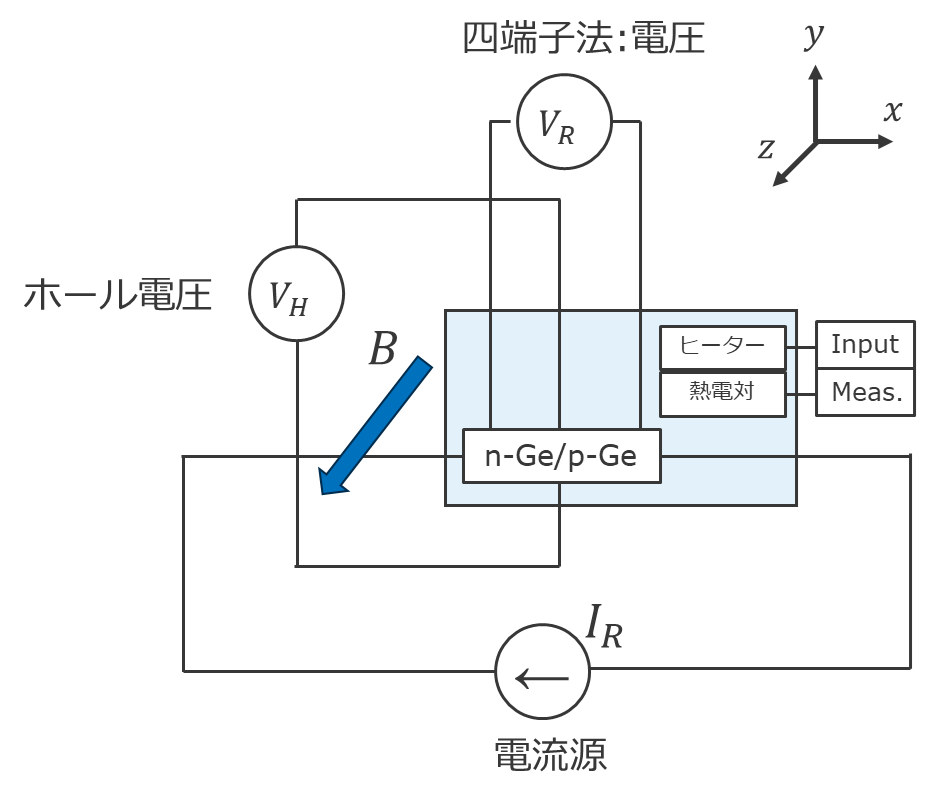
\includegraphics[width=0.4\columnwidth]{fig/fig02.png}
	\caption{\small{測定装置の模式図。ホール電圧を測定するため\(y\)軸方向に端子をつけホール電圧を測定し、
	四端子法で電気伝導度を測定する。過熱をするためのヒーターと温度計として熱電対も装置に組み込まれている。}}
	\label{fig:02}
	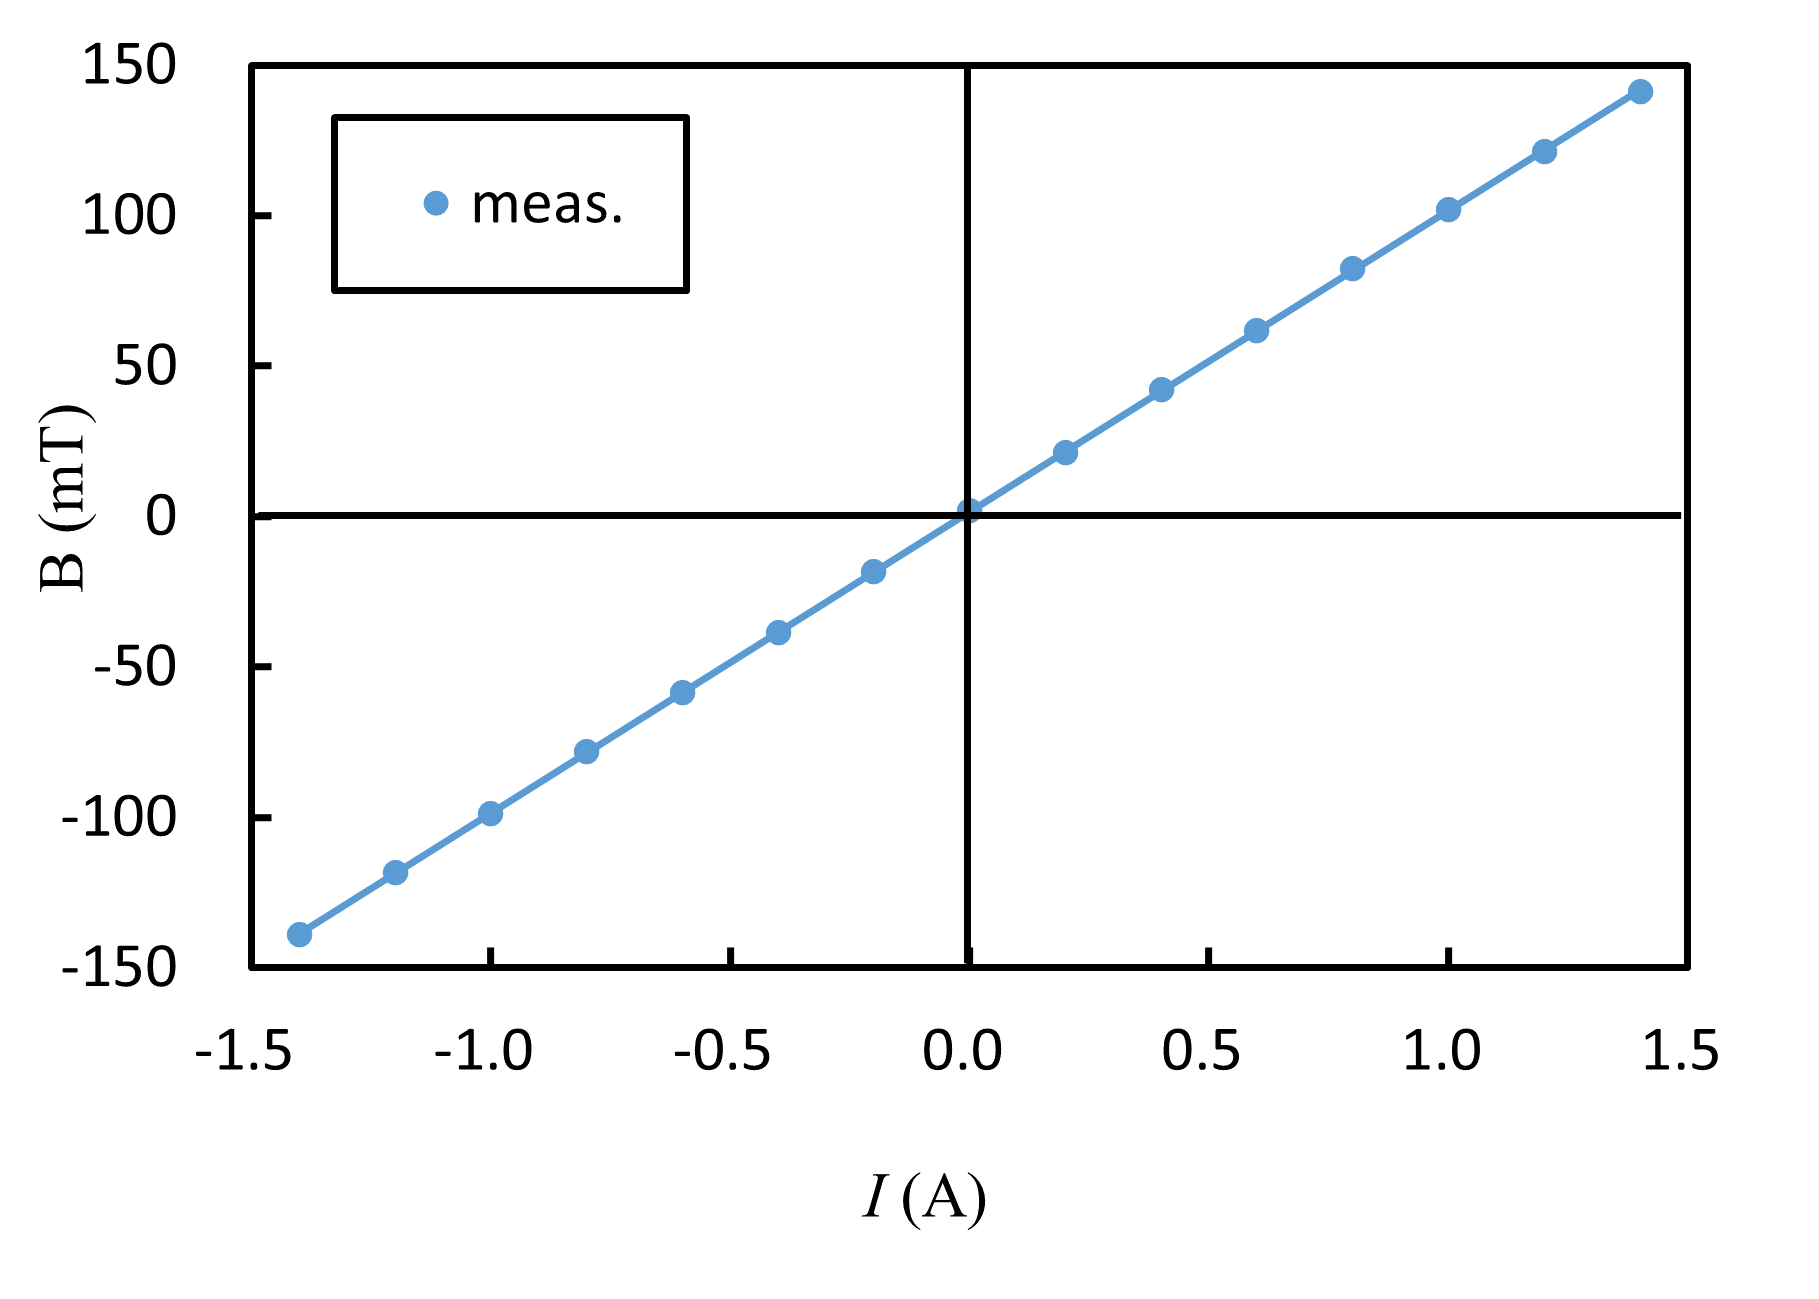
\includegraphics[width=0.4\columnwidth]{graph/graph02.png}
	\caption{電磁石に流す電流と磁場の関係の測定結果}
	\label{graph:02}
\end{wrapfigure}
\ce{n-Ge}と\ce{p-Ge}の電気伝導にかかわるパラメーターとして電気伝導度と磁場をかけたときのホール係数を試料の温度を変えながら測定した。
測定装置の模式図は図\ref{fig:02}の通りである。
半導体の電気伝導度を測定するには接触抵抗やショットキー障壁といった要素を取り除くため、4端子法で行う。
また、電流を流す方向を\(x\)軸としたときホール電圧を測定する方向を\(y\)軸として、\(z\)軸方向に電磁石によって磁場をかける。
このときホール電圧を測定する端子が\(x\)軸方向へのずれてしまうため、
測定したホール電圧はそのままではずれが生じていることに注意する必要がある。
手順としては、電流を流したときの電磁石の出す磁束密度と電流の関係の校正を行った。
その結果は図\ref{graph:02}の通りであった。この測定結果をもとに電磁石に流す電流を決めた。
試料のホール電圧の\(x\)軸方向への端子位置のずれを測定するため
-2.4 mA から 2.4 mAの直流電流を流しとゼロ磁場、室温の下で
電気伝導度とホール係数を測定した。
その後、同じ電流の範囲で \(\pm\)50 mT, \(\pm\)100 mT の磁場をかけた下でのホール電圧を測定した。
室温での測定が終わったら、ヒーターを付け試料の温度を上げていく。
1 mA の電流を試料に流しながら、ホール電圧と電気伝導度を測定した。
このとき試料のホール電圧の\(x\)軸方向への端子位置のずれの影響も考慮するため、
ゼロ磁場と 100 mT の磁場をかけたときの両方のホール電圧を測定する必要がある。

以上の測定からは試料に流す電流\(I\), 試料にかけた磁場\(B\), 試料の磁場方向の厚さ\(d\),
電気伝導度\(\sigma\), ホール電圧\(V_H\)が測定できる。
ここからわかる量として、ホール係数\(R\), キャリア密度\(n\)と\(p\), 移動度\(\mu\)が次の式よりわかる。
\begin{equation}
	R = - \frac{V_H d}{IB}, \qquad
	n = - \frac{1}{eR}, \qquad p = \frac{1}{eR}, \qquad
	\mu = \sigma R
\end{equation}

また \ce{n-Ge}に関しては低温における電気伝導度の測定を別のサンプルにて行った。(3OB 実験「電気伝導度の温度特性」)


\section{結果}

\begin{wrapfigure}[13]{r}[0pt]{0.4\columnwidth}
	\centering
	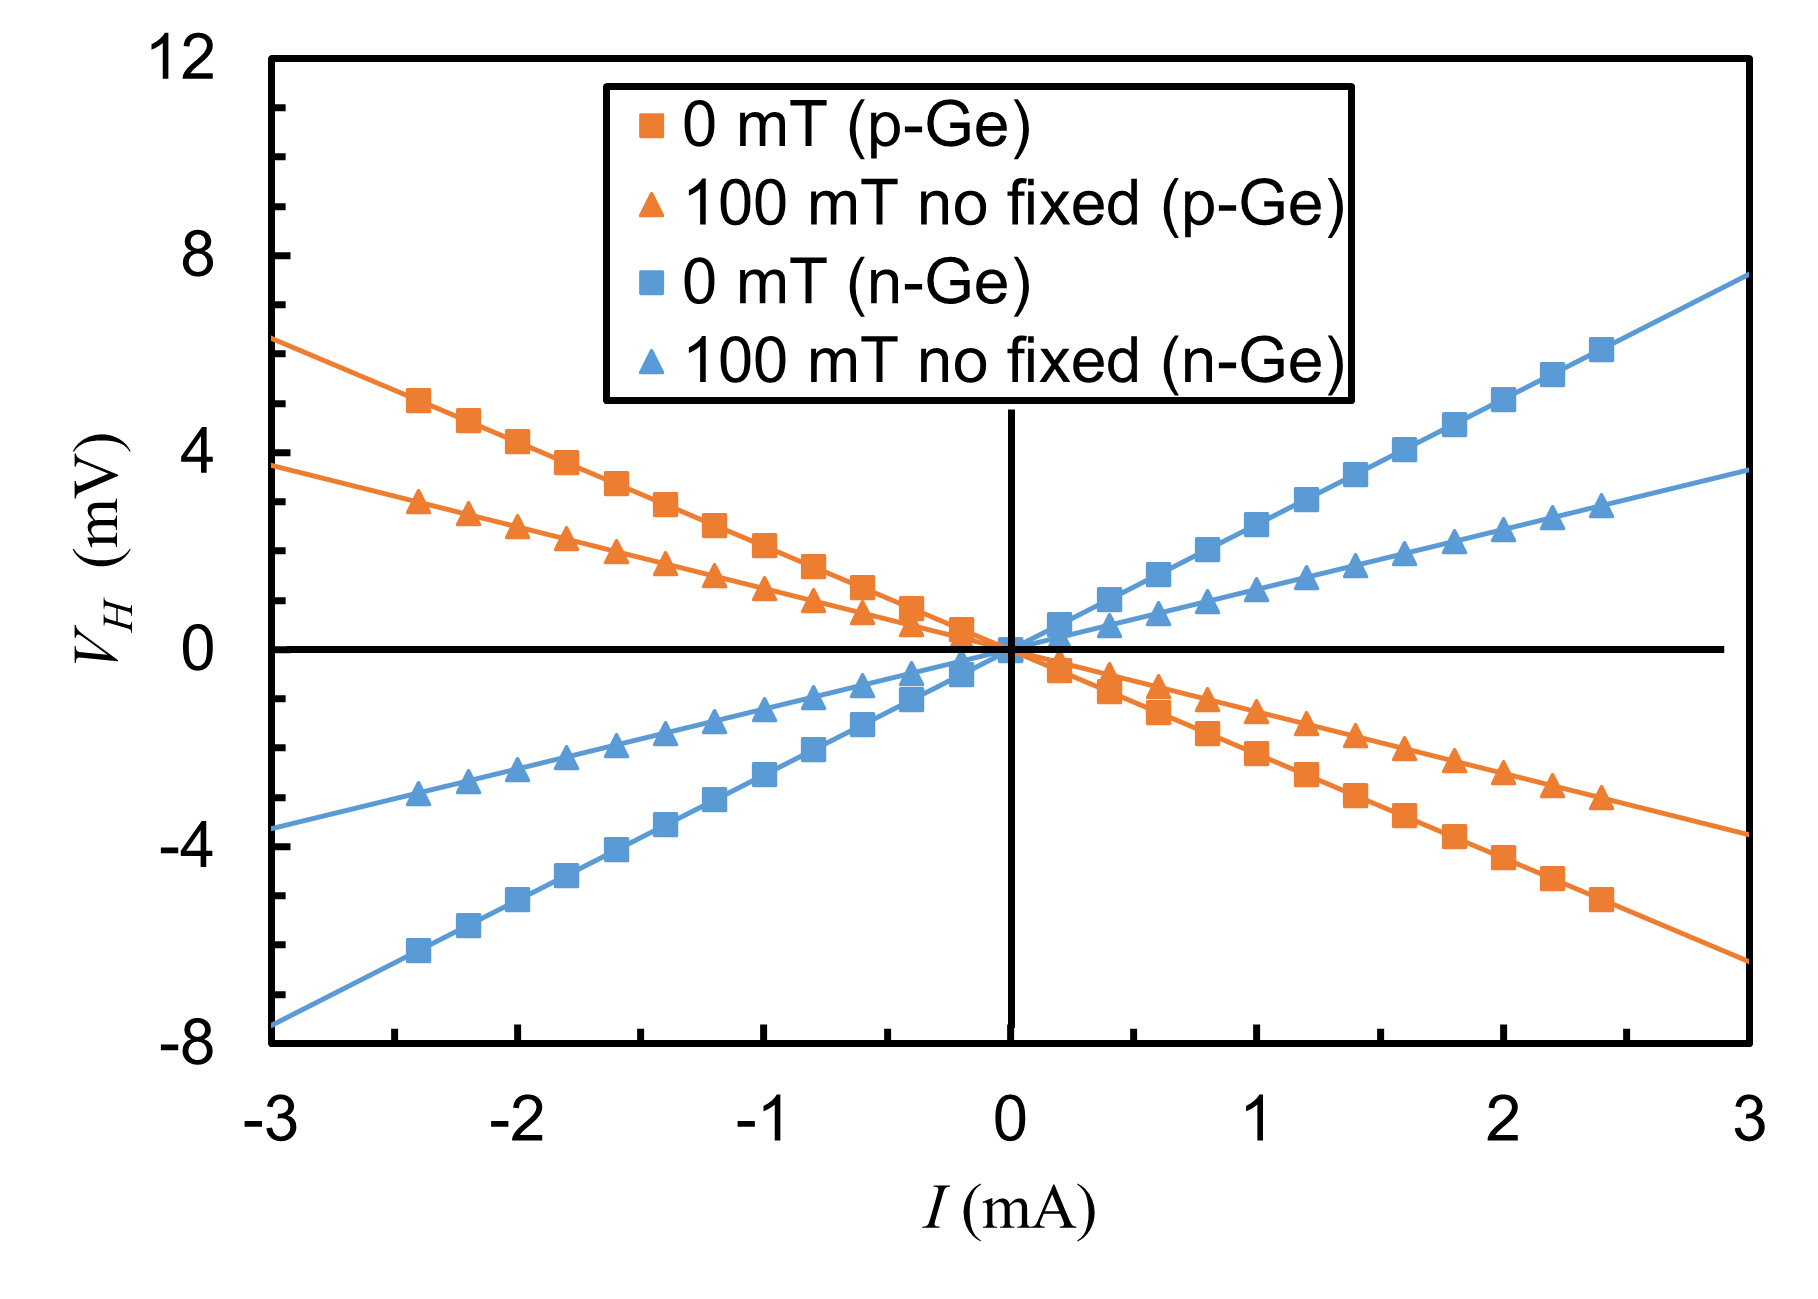
\includegraphics[width=0.4\columnwidth]{graph/graph03.png}
	\caption{試料に流した電流とホール電圧の測定結果を端子のずれの補正をせずにプロットしたもの。}
	\label{graph:03}
\end{wrapfigure}
298 K において試料に流した電流\(I\)とホール電圧\(V_H\)の間の関係は図\ref{graph:03}のようになった。
磁場\(B\)がないのにも関わらず、ホール電圧\(V_H\)が測定されてしまっているのがわかる。
これはホール電圧を測定する端子がきれいに\(y\)軸方向に取り付けられていない効果である。
なのでこの寄与を取り除いた、
298 K において試料に流した電流\(I\)とホール電圧\(V_H\)の関係は図\ref{graph:04}, 図\ref{graph:05}, 表\ref{table:01}のようになった。
確かに\(V_H \propto IB\)の関係が成り立っているのがわかる。

この実験における 298 K から 413 K における\ce{p-Ge}と\ce{n-Ge}の電気伝導度の温度特性の測定結果は図\ref{graph:09}のようになった。
また、8K から 403K までの\ce{n-Ge}の電気伝導度のアレニウスプロットは図\ref{graph:06}のようになった。
キャリアが励起に必要なエネルギーと電気伝導度の間には\(\sigma\propto \exp(-E_g/2k_B T)\)の関係より、
励起に必要なエネルギーが低温では 20 meV, 高温では 0.63 eV であることがわかる。

ホール係数\(R\)とこれの逆数によって得られるキャリア密度\(n\)と\(p\)の温度特性は図\ref{graph:07}, 図\ref{graph:08} のようになった。
\ce{p-Ge} では 70 ℃ まで、\ce{n-Ge}では 40 ℃ まで温度を上げてもキャリア数は変わらず一定になっているのがわかる。
熱励起できるキャリアがなくなった出払い領域とわかる。
出払い領域からさらに温度を上げていくとホール係数\(R\)の大きさが小さくなり、キャリア数が増えていく。
\ce{p-Ge}おいて 130 ℃を境にホール係数の符号が正から負になっているのもわかる。
これはキャリアが正孔的な性格から電子的な性格に変わったことを表す。

また、移動度の温度特性について両対数プロットしたものが図\ref{graph:10}である。
これより、\(\mu\propto T^{-3/2}\)となっている領域があるのがわかる。

\begin{figure}[H]
	\centering
	\begin{minipage}[t]{0.45\columnwidth}
		\centering
		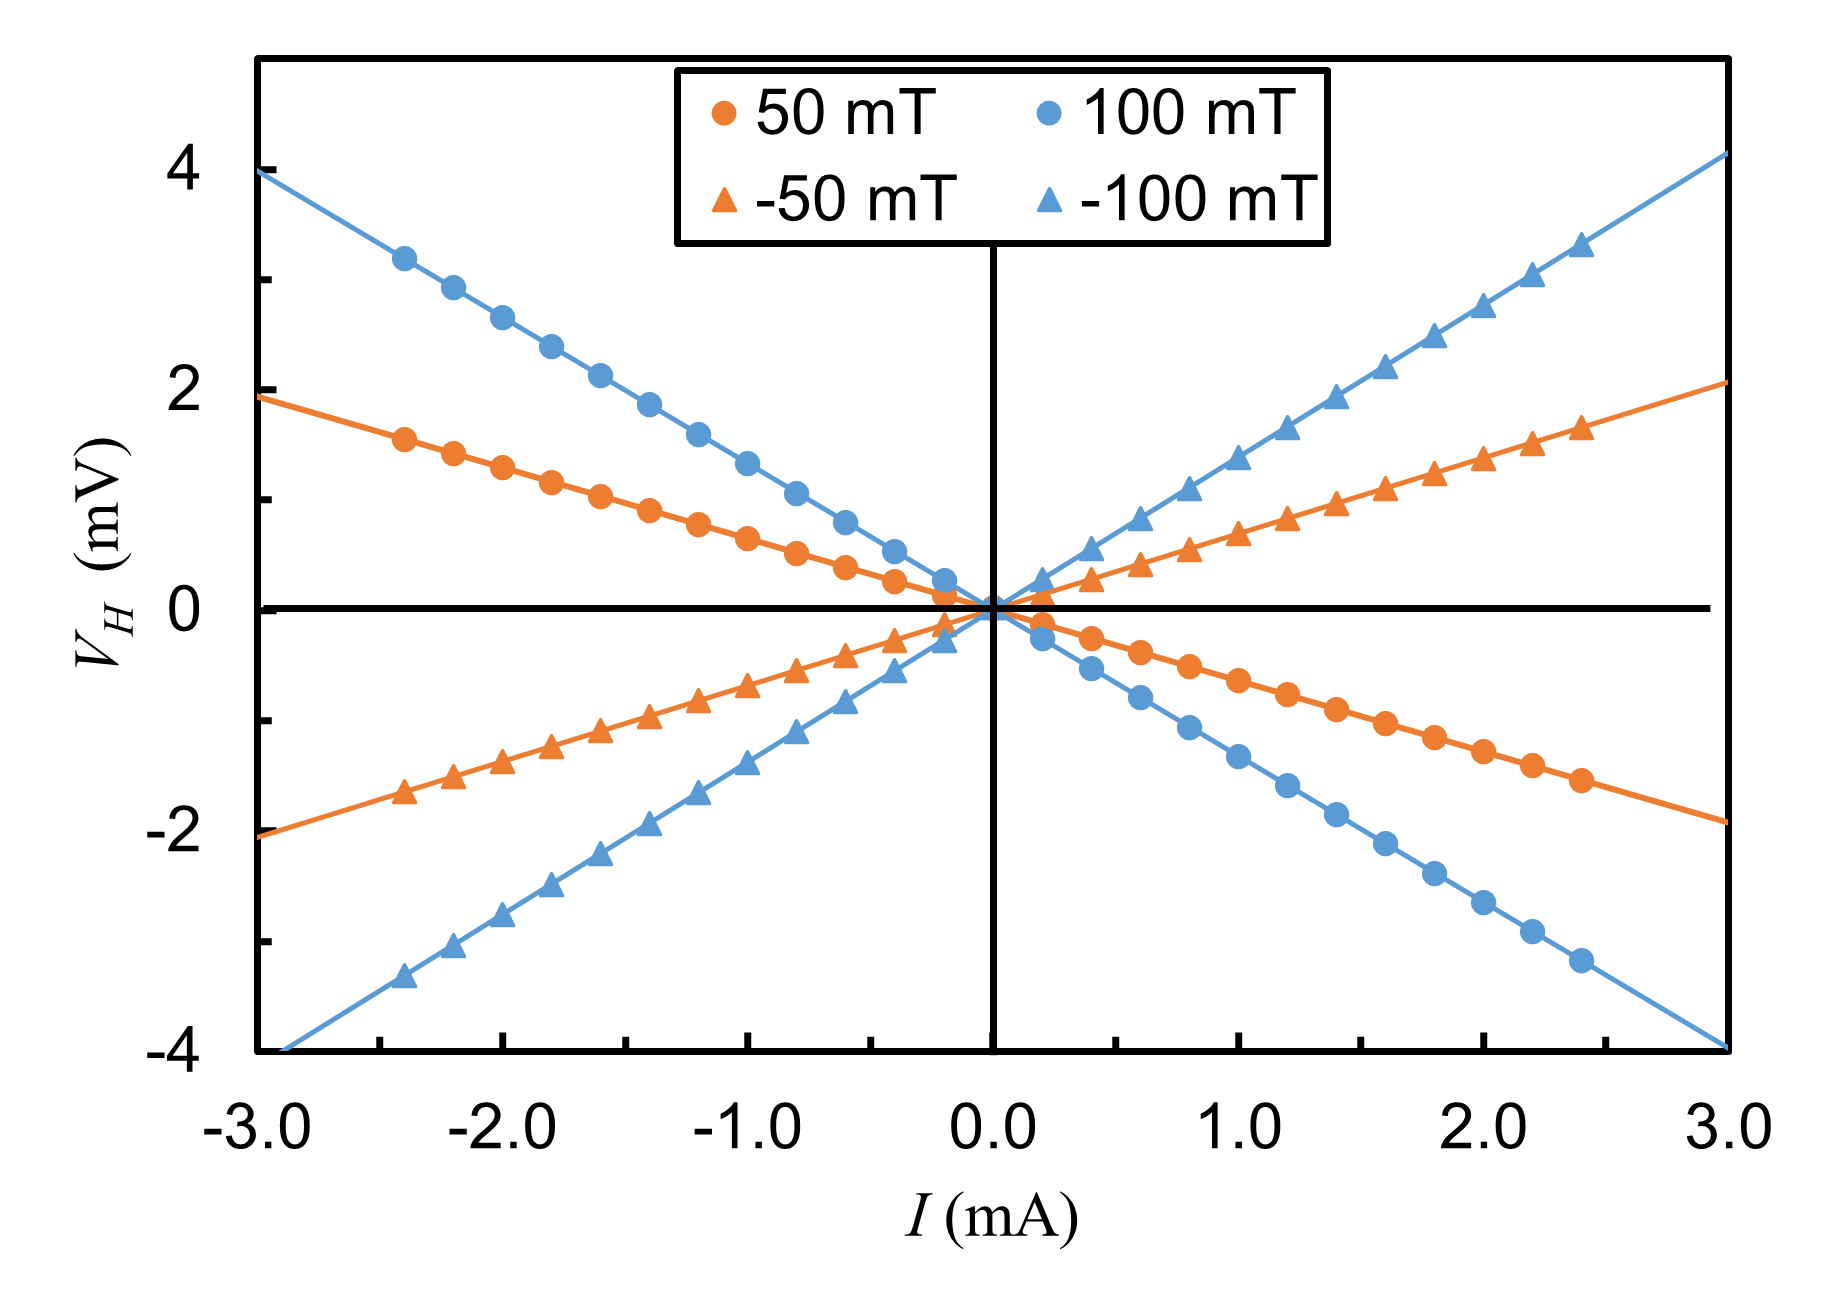
\includegraphics[width=\columnwidth]{graph/graph04.png}
		\caption{\small{298 K の室温で
		\ce{p-Ge}に流した電流\(I\)とホール電圧\(V_H\)の測定結果。(課題2)}}
		\label{graph:04}
	\end{minipage}
	\hfil
	\begin{minipage}[t]{0.45\columnwidth}
		\centering
		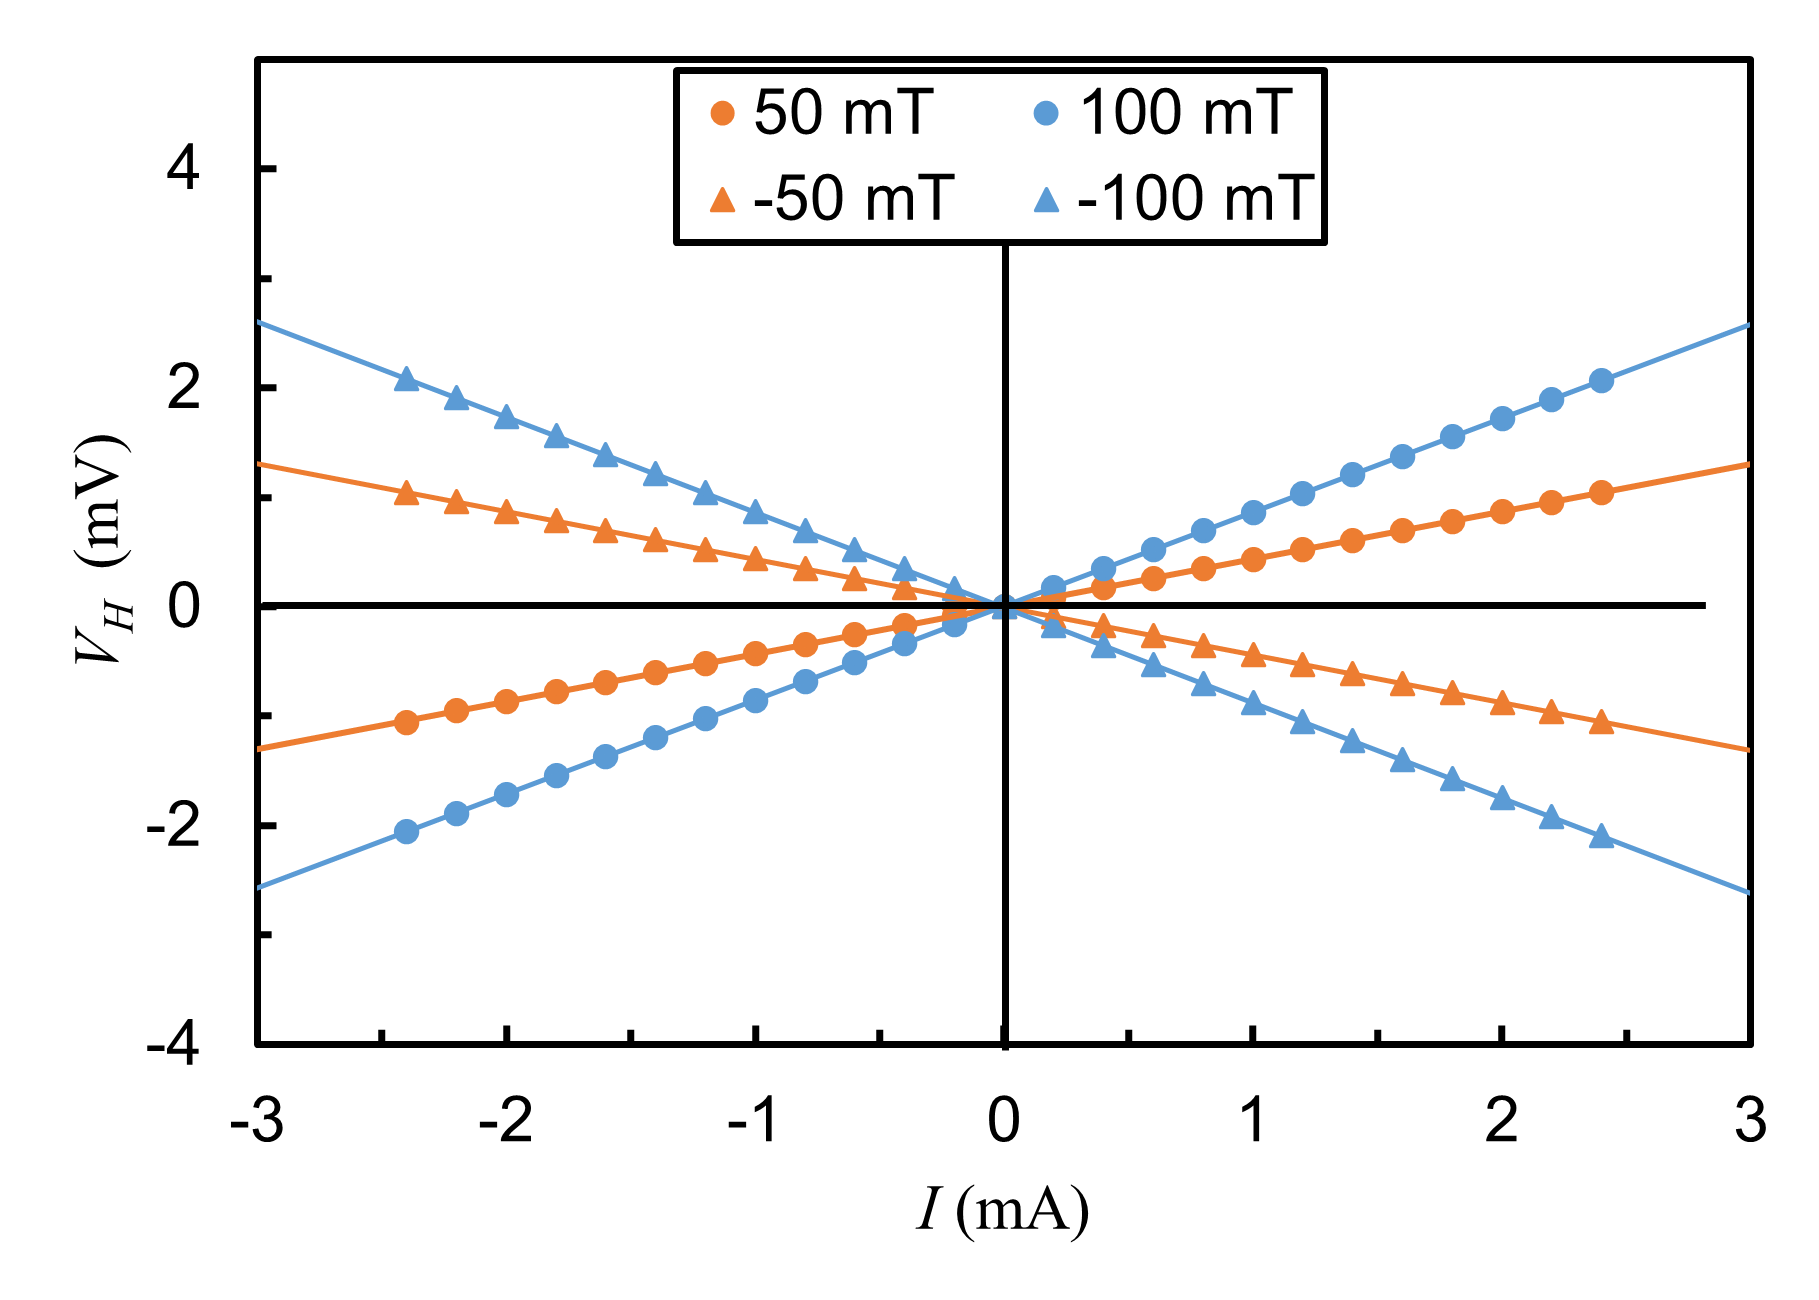
\includegraphics[width=\columnwidth]{graph/graph05.png}
		\caption{\small{298 K の室温で
		\ce{n-Ge}に流した電流\(I\)とホール電圧\(V_H\)の測定結果。(課題2)}}
		\label{graph:05}
	\end{minipage}
\end{figure}
\begin{table}[H]
	\centering
	\caption{\small{室温(298 K)におけるホール係数\(R\,(\times 10^{-3} \text{m}^3/\text{C})\),
	キャリア密度\(n,\, p\, (\times 10^{14}/\text{cm}^3)\), 移動度\(\mu\,(\times 10^{3},\,\text{cm}^2/\text{Vs})\)(課題2)}}
	\label{table:01}
	\begin{tabular}[pos]{|c|ccc|ccc|}
		\hline
		 & \multicolumn{3}{c|}{\ce{p-Ge}} & \multicolumn{3}{c|}{\ce{n-Ge}}\\
		\(B\) (mT) & \(R\) & \(p\) & \(\mu\)
		& \(R\) & \(n\) & \(\mu\)\\
		\hline
		100 & 8.59 & 7.27 & 3.48 & -13.22 & 4.71 & 3.99 \\
		 50 & 8.66 & 7.20 & 3.51 & -12.87 & 4.85 & 3.87 \\
		-50 & 8.73 & 7.15 & 3.54 & -13.75 & 4.54 & 4.14 \\
		-100 & 8.71 & 7.27 & 3.52 & -13.81 & 4.51 & 4.16 \\
		\hline
		Ave. & 8.67 & 7.20 & 3.51 & -13.42 & 4.65 &4.04 \\
		\hline
	\end{tabular}
\end{table}
\begin{figure}[H]
	\begin{minipage}[t]{0.45\columnwidth}
		\centering
		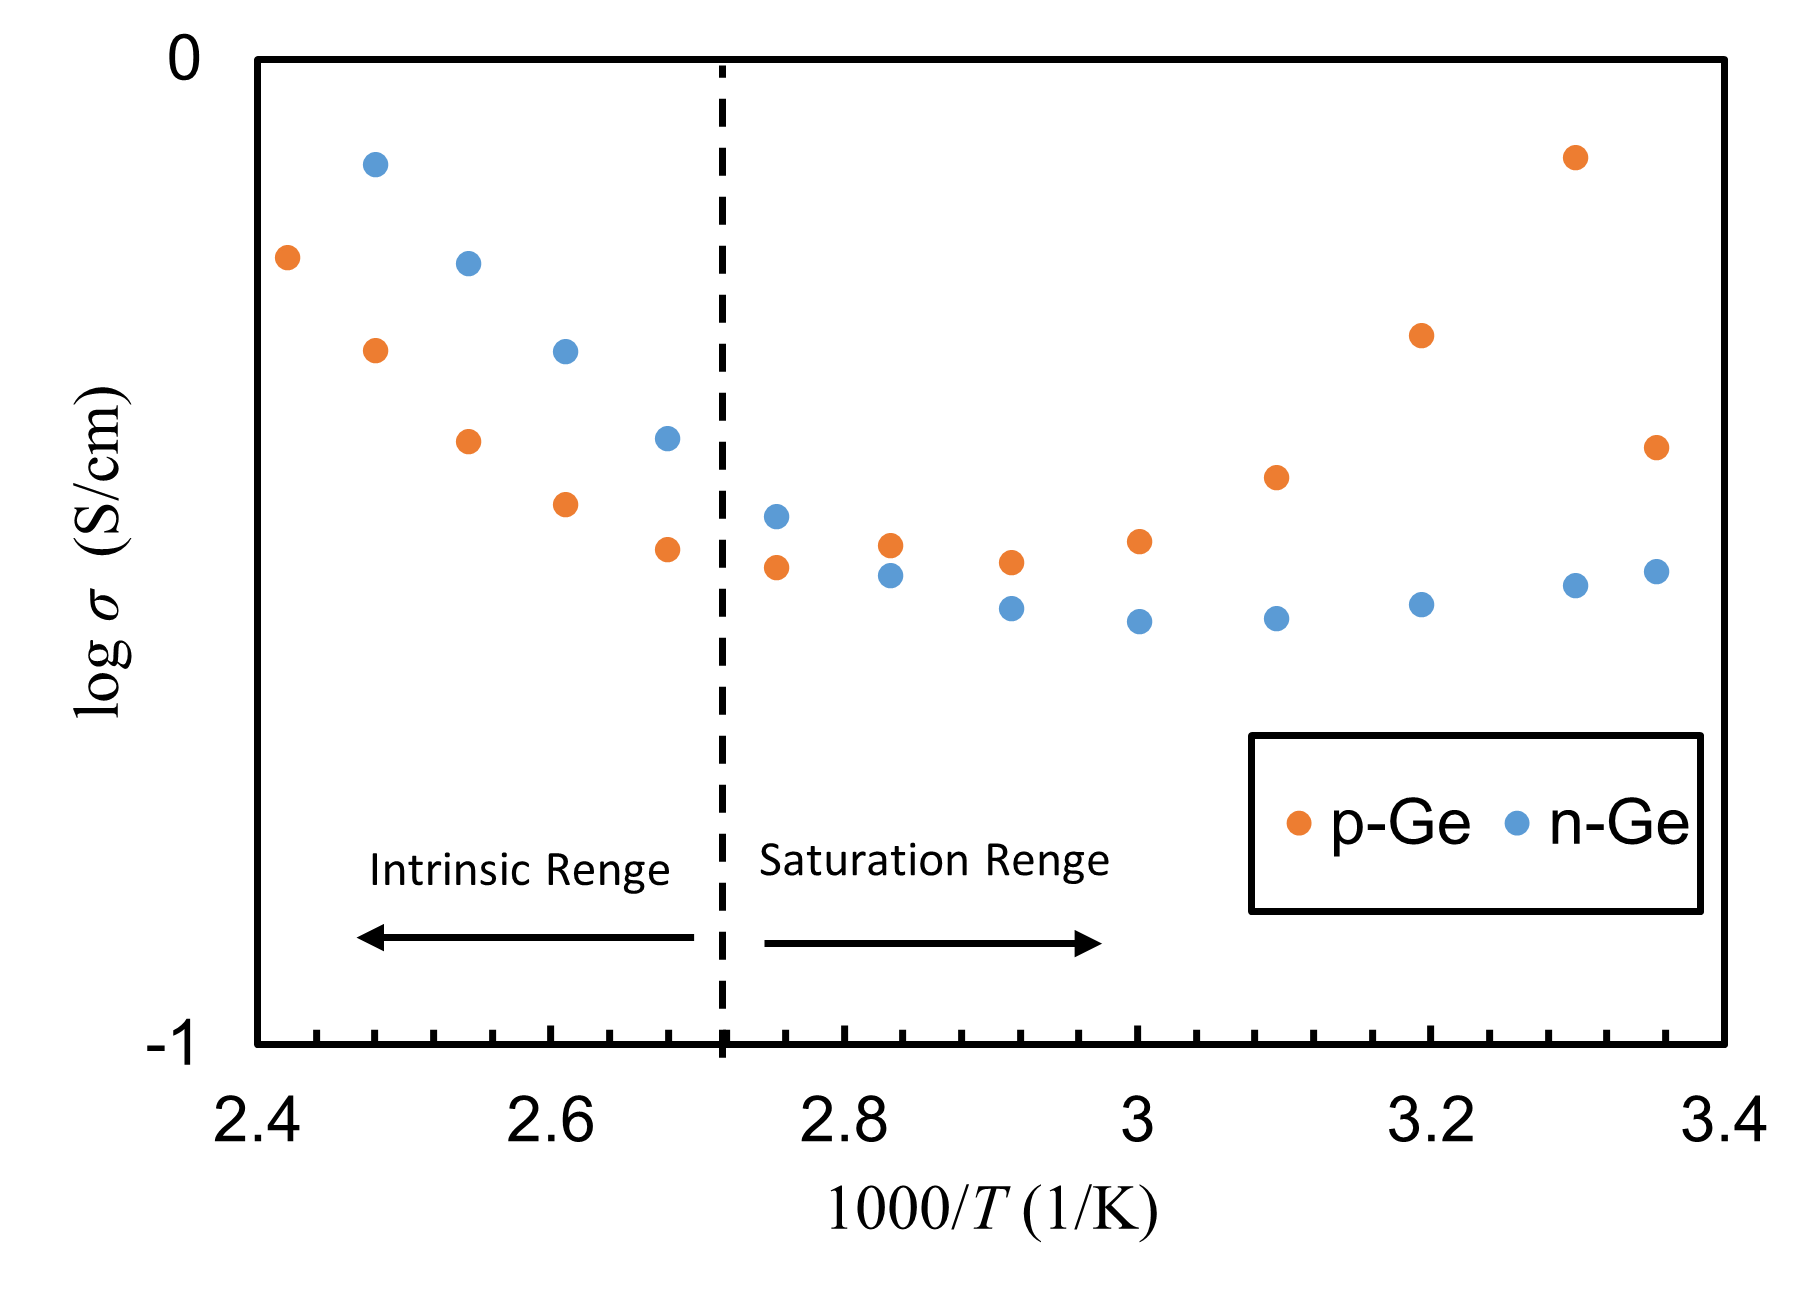
\includegraphics[width=\columnwidth]{graph/graph09.png}
		\caption{\small{\ce{p-Ge}と\ce{n-Ge}の電気伝導度の測定結果(課題4, 5)}}
		\label{graph:09}
	\end{minipage}
	\hfil
	\begin{minipage}[t]{0.45\columnwidth}
		\centering
		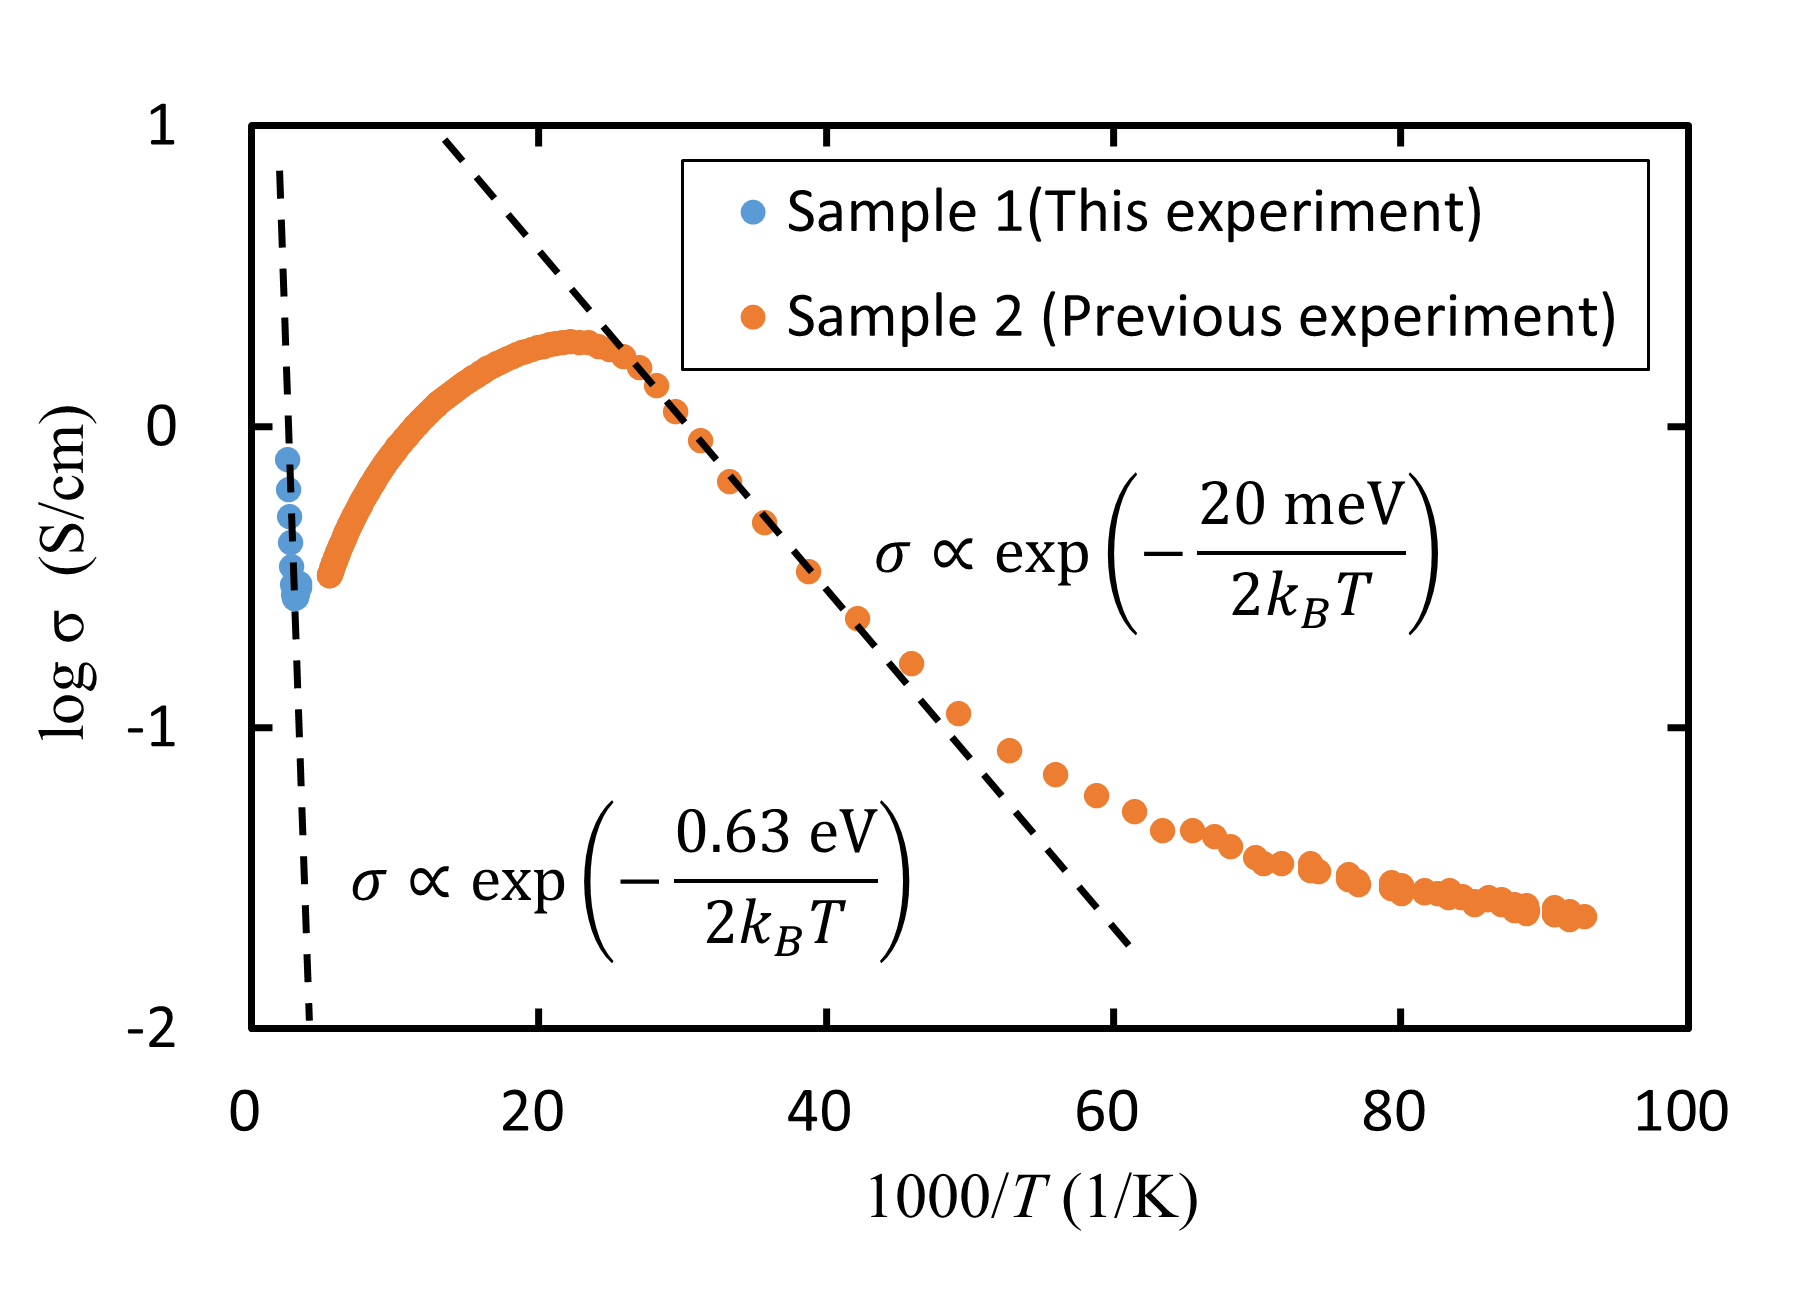
\includegraphics[width=\columnwidth]{graph/graph06.png}
		\caption{\small{\ce{n-Ge}の電気伝導度の測定結果のアレニウスプロット。
		Sample 2 は別の実験で測定したデータ。(課題4, 5)}}
		\label{graph:06}
	\end{minipage}
\end{figure}
\begin{figure}[H]
	\begin{minipage}[t]{0.45\columnwidth}
		\centering
		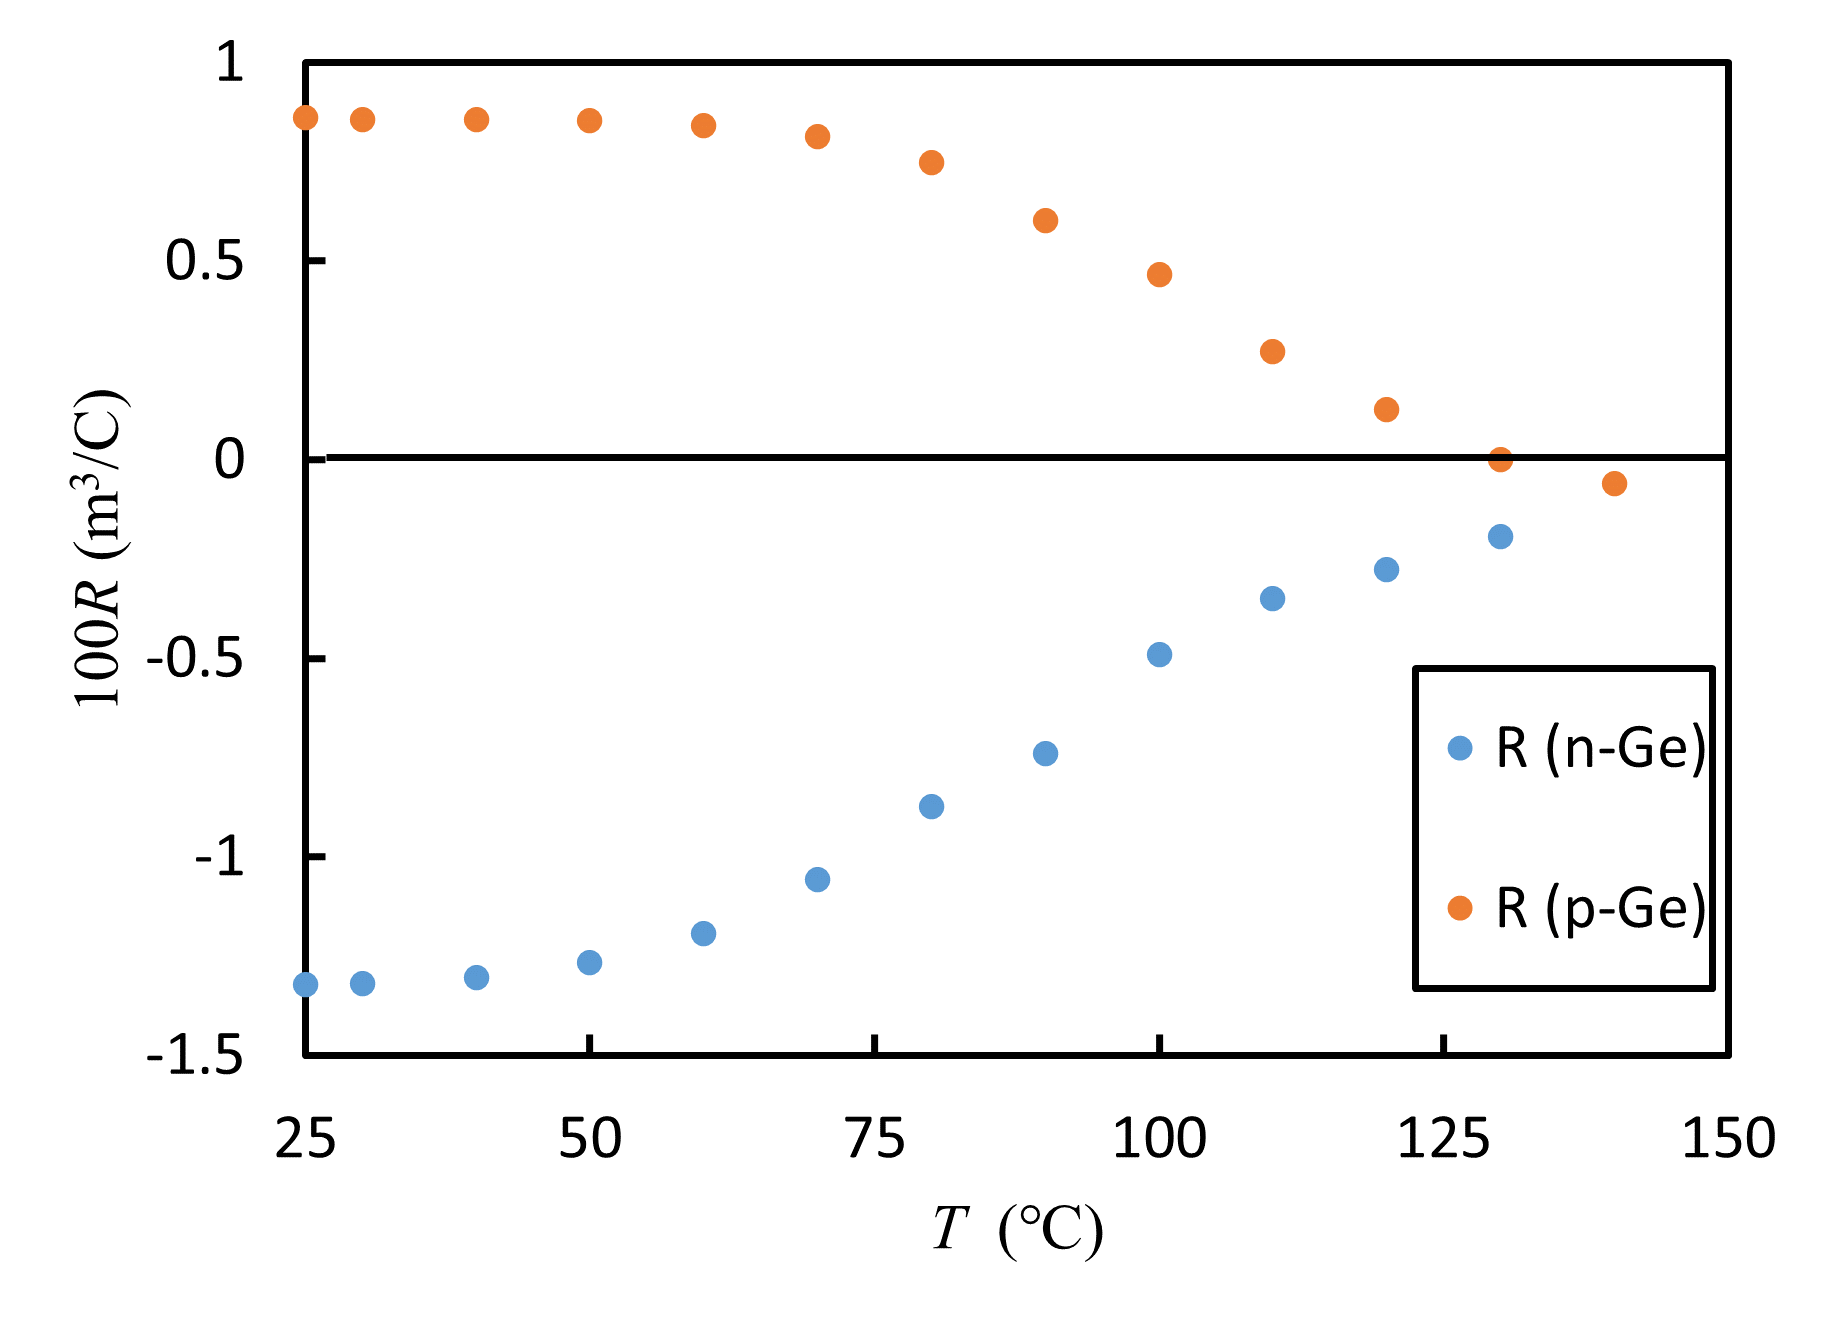
\includegraphics[width=\columnwidth]{graph/graph07.png}
		\caption{\small{ホール係数の温度特性の測定結果。
		\ce{p-Ge}が高温になると符号が正から負になっていることがわかる。(課題4)}}
		\label{graph:07}
	\end{minipage}
	\hfil
	\begin{minipage}[t]{0.45\columnwidth}
		\centering
		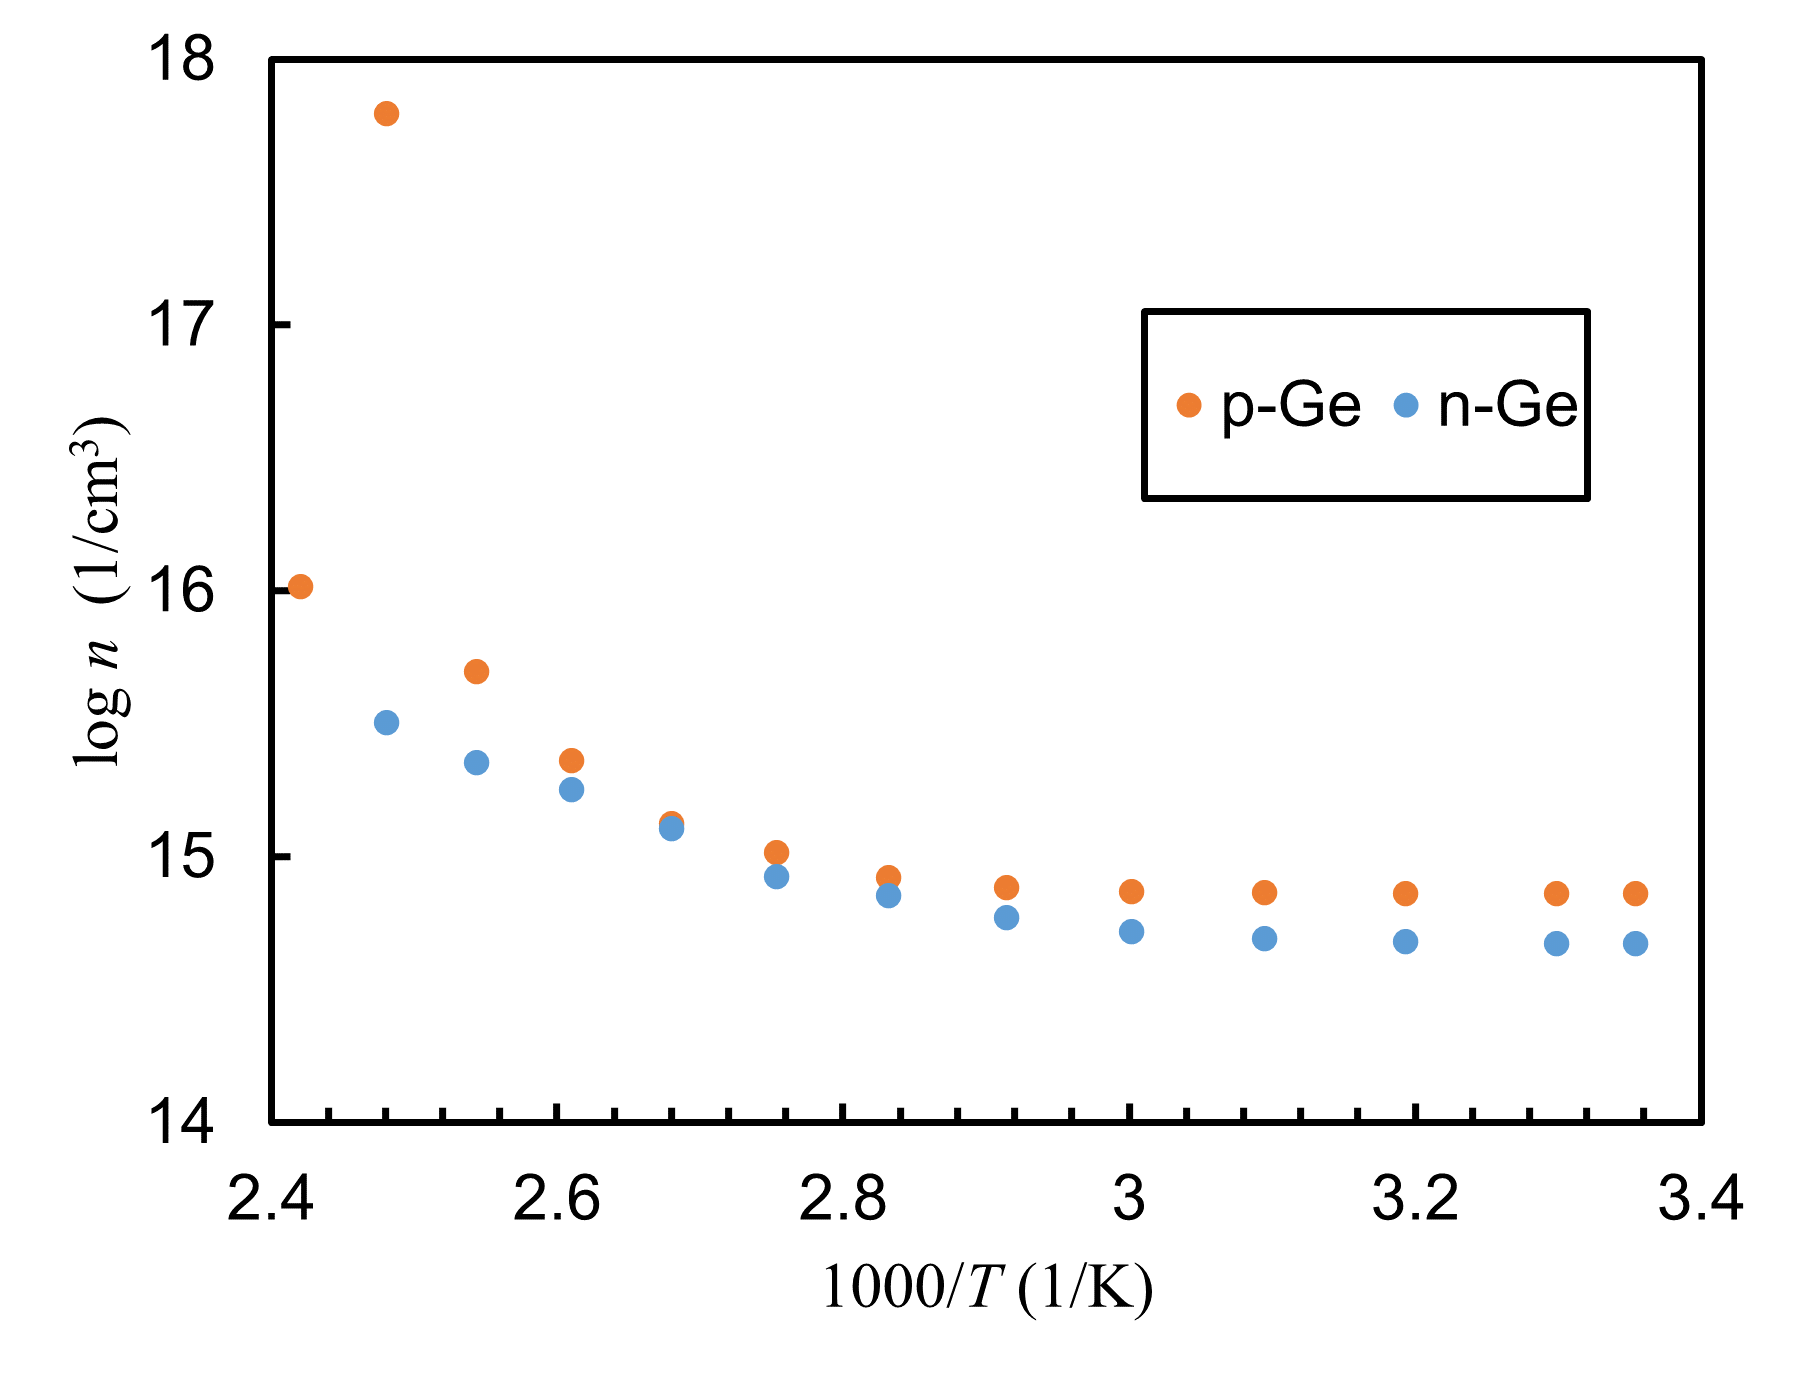
\includegraphics[width=\columnwidth]{graph/graph08.png}
		\caption{\small{ホール係数から求めたキャリア密度の温度特性。(課題7)}}
		\label{graph:08}
	\end{minipage}
\end{figure}

\begin{figure}[H]
	\centering
	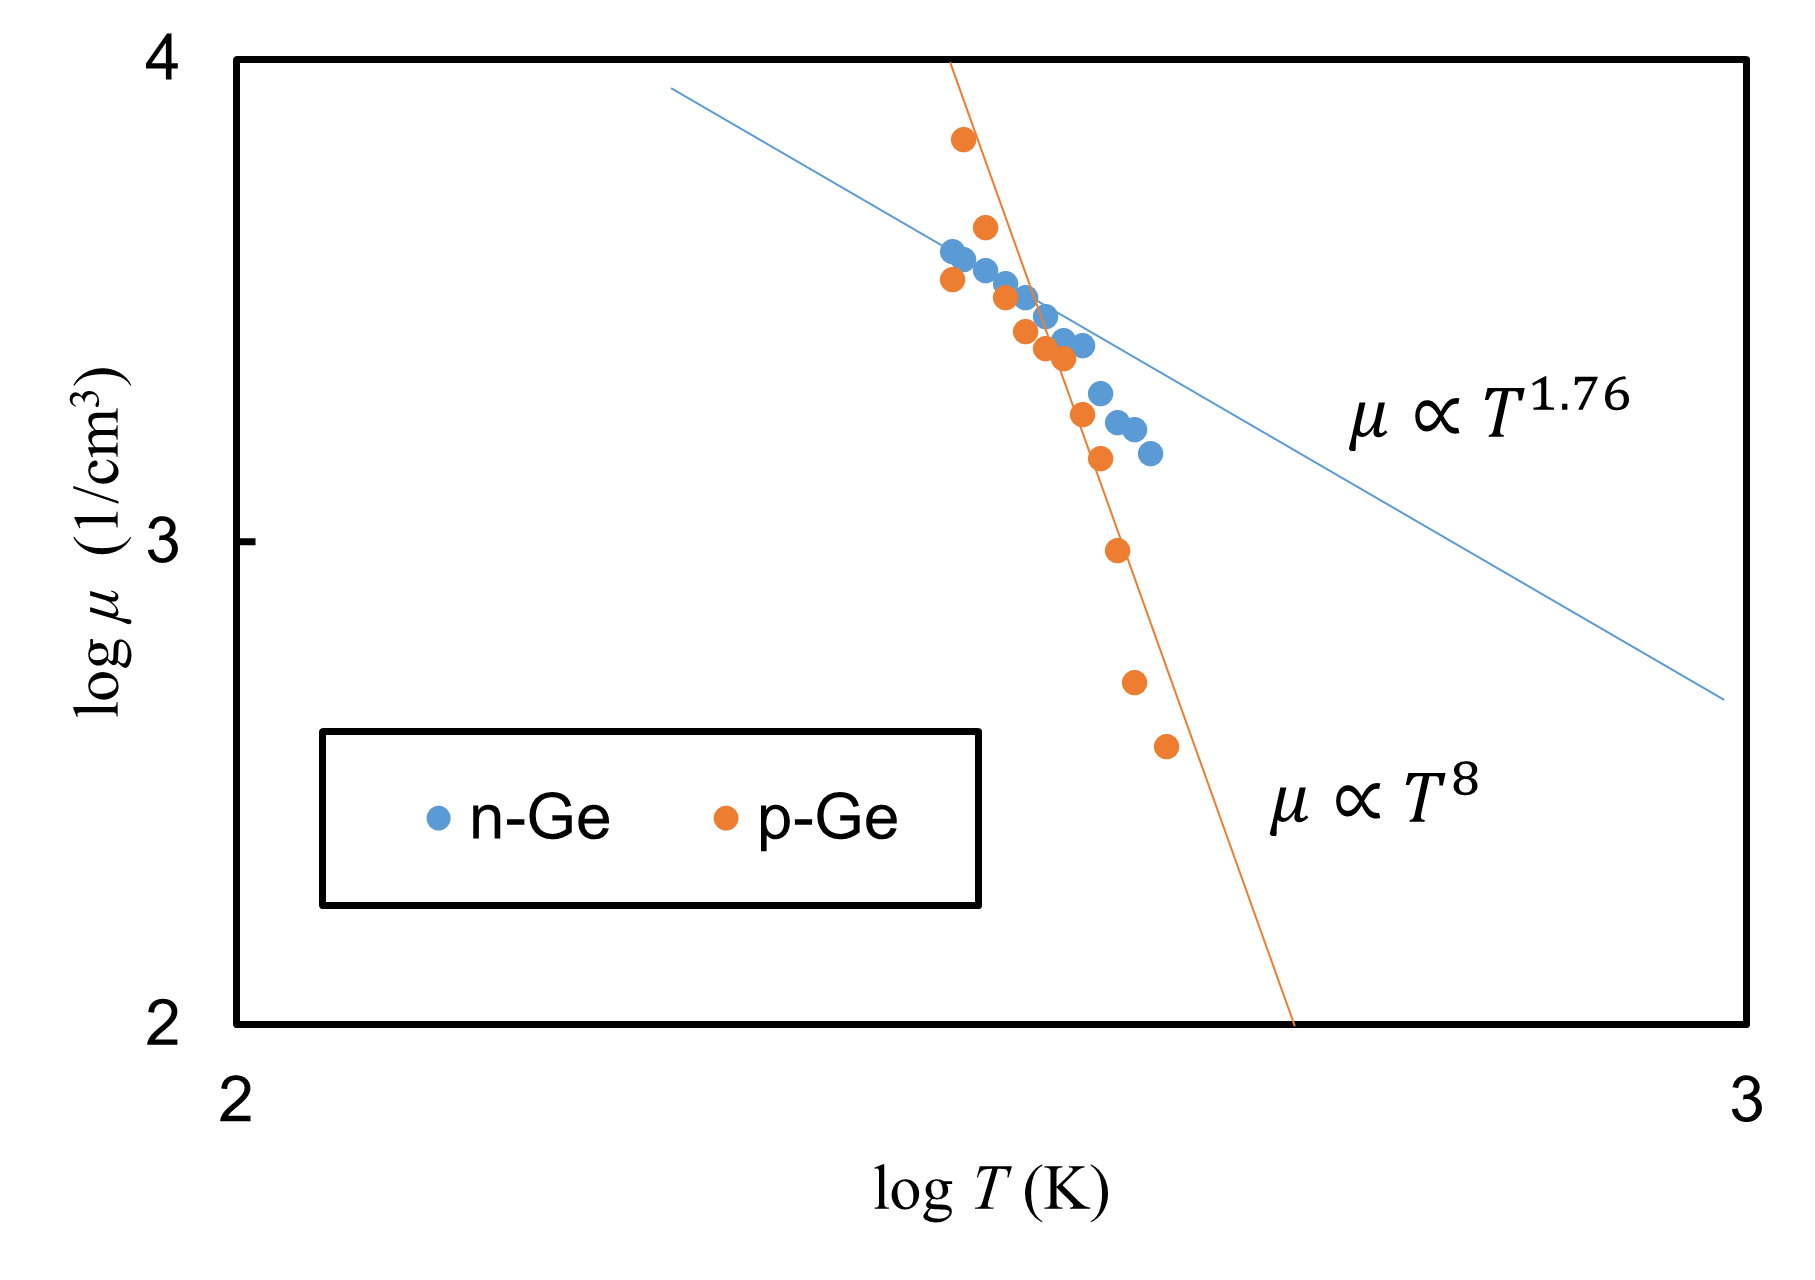
\includegraphics[width=0.49\columnwidth]{graph/graph10.png}
	\caption{\small{移動度の温度特性の測定結果を両対数プロットしたもの。(課題7)}}
	\label{graph:10}
\end{figure}

\clearpage
\section{考察}
\subsection{素励起と準粒子}
結晶中の電子の振舞いを素励起を用いた描像で考えてみる。
1つの孤立している原子を考える。
電子はその原子核に束縛され、離散的なエネルギー準位をとるようになる。
その原子が2つ近づくと、相互作用により元のエネルギー準位が分裂して2つのエネルギー準位をとるようになる。
固体中であるためこのような相互作用が多数あるため、分裂したエネルギー準位はほとんど連続的なものとみなすことができる。
これがバンドである。

そうしたバンドの準位に電子は低いエネルギーから入っていく。
その際、
パウリの排他原理によりエネルギーの低い状態となっている電子は外乱により別の状態に遷移しようとしても、
すでにほかの電子がその状態を占めているため、状態を変えることが禁じられる。
一方、エネルギーの最も高い状態付近(フェルミ面)の電子は外乱により別の状態に遷移する際に、
フェルミ面より高い準位や、他の電子がすでに励起して空になったエネルギー準位遷移することができる。

これより、結晶に外乱をいれたときに応答に関わってくるのはフェルミ面付近だけ考えばよくなる。
これはもっと言うと、フェルミ面内部にある電子は系の応答に関わらないため無視をして、
励起によりフェルミ面の外に出た電子や空になった準位だけを考えることができる。
つまり、結晶の現象はフェルミ面を新たな真空として、その真空で対生成・対消滅する電子と正の電荷をもった孔(正孔)によるものだということができる。
このような描像を素励起といい、これらにより生成・消滅する粒子を準粒子というように呼ばれる。

\begin{wrapfigure}{r}[0pt]{0.4\columnwidth}
	\centering
	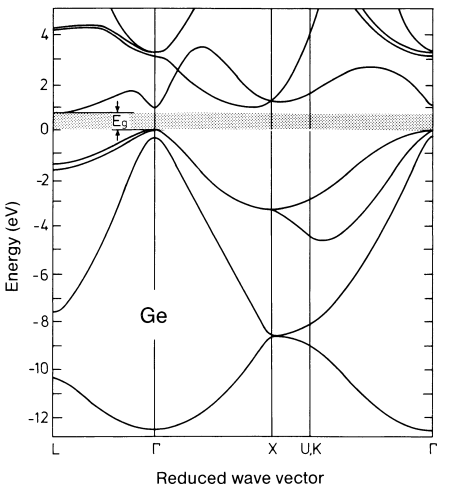
\includegraphics[width=0.4\columnwidth]{graph/graph01.png}
	\caption{Ge のバンド図\cite{ibach-luth}}
	\label{graph:01}
\end{wrapfigure}
この描像では結晶を構成する原子核の周期的ポテンシャルというのは、
準粒子の質量に取り込まれる。
このように周期的ポテンシャルを取り込んだ質量を有効質量と呼ぶ。
そのため準粒子としての電子は、
同じ電子という名前が付いているが実態としては真空中の電子とは異なり、
一定の質量をもたないような別の粒子になっている。
正孔というのも名前に孔というようにあるが、しっかりと(有効)質量をもった粒子とみなす。

有効質量は定量的にはバンドの曲率として定義される。
つまり
\begin{equation}
	\frac{1}{m_{ij}} = \frac{1}{\hbar^2}\pdv[2]{E(\vb*{k})}{k_i}{k_j}
\end{equation}
として定義される。
波数空間が等方的であるときには有効質量はテンソル量ではないスカラー量
\begin{equation}
	\frac{1}{m} = \frac{1}{\hbar^2}\pdv[2]{E(\vb*{k})}{k}
\end{equation}
となる。
有効質量によって周期的ポテンシャルというのは準粒子の運動方程式に現れなくなり、
自由粒子と同じ運動方程式となる。なので準粒子は固体内部で理想気体のように振舞う。

実際の Ge のバンド図(図\ref{graph:01})との対応を見てみる。
フェルミ面がバンドギャップ\(E_g\)の間を通っている結晶は半導体と呼ばれる。
実際に電子と正孔の対生成・対消滅する場所としては Reduced wave vector が \(\Gamma\)
つまり波数ベクトルが\(\vb*{k}=(0,\,0,\,0)\)の地点にあるエネルギーギャップ付近である。
上下に放物線があり、上にある放物線上に準粒子としての電子が現れ、下にある放物線上に正孔が現れる。
このとき正孔は真空より低い負のエネルギーを持っているように見えるが、
そのようにとらえるのではなく符号を取り直して正のエネルギーを持つものと考える。
\footnote{Dirac が考えた Dirac の海による陽電子の説明と似ている。
歴史的には Peierls が1929年に電子と正孔を用いて Holl 効果を説明してから Dirac の海の話が1930年に出たようである。
Dirac の海による陽電子の予言の偉いところは Dirac の海のような描像を思いつた点ではなく、
電子と正孔の生成というのがフェルミ面という"真空"で粒子が対生成・対消滅していて、
真空でもこれと同様なことを思いついた点であるのだろう。ただこの話の証拠はないため私の妄想ではある。}
フェルミ面を真空としているので、フェルミ面のエネルギーを 0 とすると\footnote{図\ref{graph:01}の縦軸のエネルギーの基準点とは違う基準}、
この放物線はそれぞれ、
\begin{equation}
	E(k) = E_e + \frac{\hbar^2k2}{2m_e^*}, \qquad
	E(k) = -\qty(E_p + \frac{\hbar^2k2}{2m_p^*})
\end{equation}
となる。ここで\(E_e,\,E_p\)を電子と正孔の生成エネルギー、\(m_e^*,\,m_p^*\)を電子と正孔の有効質量とした。
電子・正孔の分散関係と呼ばれ、分散関係がわかるとエネルギーの幅が\([E,\,E+dE]\)の間にとることのできる状態の数を表す(有効)状態密度\(D(E)dE\)というのも求められる。

エネルギー\(E(k)\)における状態密度は粒子の生成エネルギーを\(E_s\)として
\begin{align}
	D(E)
	&= 2\times\sum_k \delta(E-E(k)) \notag\\
	&= \frac{2V}{(2\pi^3)}\int d\vb*{k}\, \delta\qty(E-E_s - \frac{\hbar^2k^2}{2m^*}) \notag\\
	&= \frac{V}{\pi^2} \int dk\, k^2\times \frac{1}{2}\sqrt{\frac{\hbar^2}{2m^*(E-E_e)}}\qty{\delta\qty(k-\sqrt{\frac{2m^*(E-E_s)}{\hbar^2}})+\delta\qty(k+\sqrt{\frac{2m^*(E-E_s)}{\hbar^2}})} \notag\\
	&= \frac{V}{2\pi^2}\qty(\frac{2m^*}{\hbar^2})^{3/2}\sqrt{E-E_s}
\end{align}
として求められる。

また、粒子の分布関数はフェルミ分布関数で表される。
しかし、\(E_e,\, E_p \simeq \text{eV} \simeq 10^4 \text{K}\)であることから、
\num{e4} K のような高温でない限り、フェルミ分布関数をボルツマン分布とみなしてよい。
\begin{equation}
	f(E) = \frac{1}{1+e^{E/k_BT}} \simeq e^{-E/k_BT}
\end{equation}
これより電子と正孔の密度は
\begin{align}
	n &= \int_{E_e}^\infty D_e(E) f(E) dE = 2\qty(\frac{m_e^*k_BT}{2\pi\hbar})^{3/2}e^{-E_e/k_BT}\\
	p &= \int_{E_p}^\infty D_p(E) f(E) dE = 2\qty(\frac{m_p^*k_BT}{2\pi\hbar})^{3/2}e^{-E_p/k_BT}
\end{align}
となる。
この式から質量作用の法則と呼ばれる式
\begin{equation}
	pn = 4\qty(\frac{k_B T}{2\pi\hbar})^3\qty(m_p^*m_n^*)^{3/2} e^{-E_g/k_BT}
\end{equation}
が得られる。
結晶内での電荷中性条件\(p=n\)より
\begin{equation}
	p=n=2\qty(\frac{k_B T}{2\pi\hbar})^{3/2}\qty(m_p^*m_n^*)^{3/4} e^{-E_g/2k_BT} \label{eq:5-9}
\end{equation}
が得られる。
電荷中性条件から別の式を得ることができる。
\(p/n=1\)より
\begin{align}
	1 &= \qty(\frac{m_p^*}{m_e^*})^{3/2}e^{-(E_p-E_c)/k_BT}\\
	E_p - E_n &= \frac{3}{2}k_BT\ln(\frac{m_p^*}{m_e^*})
\end{align}
\(E_g = E_p + E_n\)と合わせて考えると
\begin{equation}
	E_p = \frac{E_g}{2} + \frac{3}{4}k_BT\ln(\frac{m_p^*}{m_e^*}), \qquad
	E_n = \frac{E_g}{2} + \frac{3}{4}k_BT\ln(\frac{m_n^*}{m_p^*})
\end{equation}
という式が得られる。
低温であれば\(E_p=E_n=E_g/2\)であることがわかり、
温度を上げていくと有効質量の大小によって正孔と電子の生成エネルギーに差ができることがわかる。
\ce{Ge}ではバンド図(図\ref{graph:01})より\(m_e^* < m_p^*\)であるため正孔の方が大きい。

通常のバンド理論ではフェルミ面より下にあるバンドを価電子帯、上にある伝導帯と呼ばれる。
この呼び方は次のような描像から来ている。
価電子帯と呼ばれるバンドの内部にある電子は、
上の説明からわかるように電気伝導にかかわることはない。
その理由をこの電子は原子核に束縛されて動けない価電子であるからだというように考える。
一方、伝導体と呼ばれるバンドの内部にある電子は素励起による説明における電子になっている。
するとその電子は束縛されていない自由電子で、結晶内を移動していくキャリアとなる。
なので価電子帯や伝導帯のように呼ばれている。
また、正孔にとってはフェルミ面の上側にあるのが価電子帯、下側にあるのが伝導帯となる。

\subsection{半導体への不純物ドーピング}
Ge 半導体に原子番号が隣の元素である \ce{As} か \ce{Ga} の一方を少量だけ混ぜることを考える。
まず初めに \ce{As} を1つだけ加えることを考える。
素励起の描像では \ce{Ge} の結晶だけでは真空であったので、
もともとの \ce{Ge} 結晶からの差分だけが系にあるとみなせる。
\ce{As} の原子核の持つ正電荷は\ce{Ge}の原子核と比較するとだいたい1つ増え、電子が1つ増える。
つまり水素原子と同じ系になっている。
よって新しく追加された電子のシュレーディンガー方程式は
\begin{equation}
	\qty(-\frac{\hbar^2}{2m_e^*}\laplacian - \frac{e^2}{4\pi\varepsilon r})\psi = E \psi
\end{equation}
となる。ここで、\(\varepsilon\)は\ce{Ge}結晶の誘電率である。
\ce{As} に束縛された電子は\ce{Ge}の電子の分散曲線に励起すると自由電子となることから、
エネルギーは伝導体の下端をエネルギーの基準とした
\begin{equation}
	E_n = E_e - \frac{m_e^*}{2\hbar^2}\qty(\frac{e^2}{4\pi \varepsilon})^2\frac{1}{n^2}
\end{equation}
というようになる。
追加する不純物は少量であるため、不純物間の間は十分離れてるとみなせる。
なのでこれによるバンド分裂は細くてないものとみなせる。
もともとのエネルギーは eV オーダーの量にたいして、
不純物によってできた新たな準位による束縛エネルギーは meV オーダーである。
これより極端な低温ではないかぎり、熱よって励起をすることができる。
そうして熱励起した電子はキャリアとして半導体内を動くようになる。
なのでキャリアの符号からこれをn型半導体という。

そして\ce{Ga}を加えたときのことを考える。
もともとの \ce{Ge} 結晶からの差分だけが系にあるとみなせる。
\ce{Ga} の原子核の持つ正電荷は\ce{Ge}の原子核と比較するとだいたい1つ減り、電子が1つ減る。
これはつまり、負の電荷をもった原子核の周りに正の電荷をもった正孔があるという水素原子と同じ系となる。
なので\ce{As}のときと同様に考えて
\begin{equation}
	E_n = E_p - \frac{m_e^*}{2\hbar^2}\qty(\frac{e^2}{4\pi \varepsilon})^2\frac{1}{n^2}
\end{equation}
というようなエネルギー準位が表れ、
熱により、正孔がキャリアとして励起することができる。
これをp型半導体という。

不純物が入っていない半導体を真性半導体という。
これら3つの簡略化したバンド図は図\ref{fig:01}のようになる。 % TODO もっと説明書く
\begin{figure}[h]
	\centering
	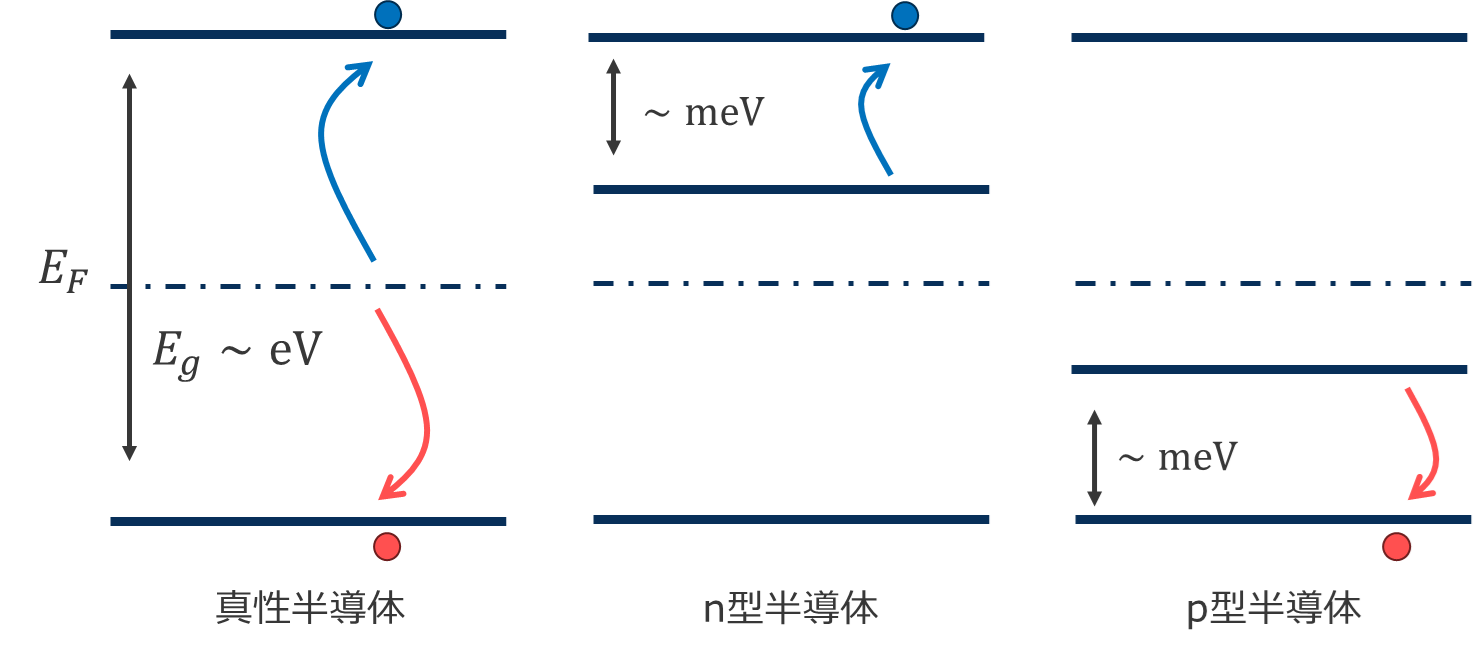
\includegraphics[width=0.65\columnwidth]{fig/fig01.png}
	\caption{不純物を入れたときの簡略化したフェルミ面付近のバンド図}
	\label{fig:01}
\end{figure}

\section{課題}
\begin{tcolorbox}[title=課題1]
	半導体に比べ、金属のホール測定が難しい理由を考察せよ。
\end{tcolorbox}
ホール係数は
\begin{equation}
	V_H = -\frac{1}{nq} \frac{IB}{d} = -R\frac{IB}{d} \tag*{(\ref{eq:2-15})式再掲}
\end{equation}
として表わされる。
また、電子や正孔の粒子数は
\begin{equation}
	p=n=2\qty(\frac{k_B T}{2\pi\hbar})^{3/2}\qty(m_p^*m_n^*)^{3/4} e^{-E_g/2k_BT} \tag*{(\ref{eq:5-9})式再掲}
\end{equation}
である。金属では\(E_g=0\)であるので、
同じ温度の元、電子と正孔の質量が同じものとすると、これらの式から半導体と金属のホール係数の比は
\begin{equation}
	\frac{R_{\text{metal}}}{R_{\text{semi conductor}}}  = e^{-E_g/k_BT}\simeq 10^{-9}
\end{equation}
となる。
最後の等号は\(E_g\simeq 10^4 \text{K}\)としてオーダーを見積もったものである。
半導体と金属で同じ形状をしているとしたら、
このことはホール電圧が\num{e-9}倍小さい値で測定されることを表している。
なので金属のホール係数を測定することはこの系では難しいことがわかる。
\\

\begin{tcolorbox}[title=課題2]
	\(\Delta V_H\)からホール係数\(R\)を導出し、
	主たるキャリアの種類を判定せよ。
	さらに、試料の電気電伝導度\(\sigma\)と併せてキャリア密度\(n\)と移動度\(\mu\)を算出せよ。
\end{tcolorbox}
室温(298K)におけるホール係数\(R\), キャリア密度\(n,\, p\), 移動度\(mu\)は
図\ref{graph:04}, 図\ref{graph:05}, 表\ref{table:01} にて示した。
それより高温領域のホール係数\(R\)は図\ref{graph:07}, キャリア密度は図\ref{graph:08}, 移動度\(\mu\)は図\ref{graph:10},
電気伝導度は図\ref{graph:09}, 図\ref{graph:06} に示した。

この結果より\ce{n-Ge}では電荷が負のキャリアである電子が優勢であることがわかる。
また\ce{p-Ge}では 130 ℃ 未満では電荷が正のキャリアである正孔が、
130 ℃ 以上ではキャリアが負である電子が優勢であることがわかる。
\\

\begin{tcolorbox}[title=課題4]
	\ce{p-Ge}のホール係数\(R\)の温度変化を考察せよ。
\end{tcolorbox}

電気伝導のキャリアが2種類あるためホール係数\(R\)は
\begin{equation}
	R = \frac{p\mu_p^2 - n\mu_e^2}{e(p\mu_p+n\mu_e)^2} \tag*{(\ref{eq:2-23})式再掲}
\end{equation}
はとして表される。
つまり、ホール係数の逆数をもとにキャリア密度をプロットした図\ref{graph:08}では、
キャリアの様子を考えるのには不適切である。
キャリア密度は散乱の寄与があるものの電気伝導度\(\sigma\)に比例することから、
図\ref{graph:09}を用いて考えるのがよい。

60 ℃付近まではホール係数\(R\)が一定でであり、
電気伝導度\(\sigma\)も大きな変化はないことがグラフより確認できる。
これはアクセプタ準位に不純物によって供給された正孔が大方、
励起したことによってキャリア数が変化しないという状態になっていると考えられる。

そこから温度を上げていくとホール係数\(R\)は下がって行き、
130 ℃ ではホール係数\(R\)の符号が正から負に反転している。
これはホール係数\(R\)の分子の値が徐々に減っていってることを示唆する。
また電気伝導度\(\sigma\)は増えていってるのがわかる。
これはキャリア密度の増加を表している。
この振る舞いは温度を上げることでアクセプタ準位にある正孔だけでなく、
対生成した電子・正孔がキャリアとして動くようになったからというので説明できる。

ドープした不純物の量は少ない。
そのため、アクセプタ準位にある正孔の数よりも対生成した電子・正孔の数が温度\(T\)を上げるにつれ多くなっていく。
なので対生成した電子・正孔だけを考えればよい。
電荷中性条件より\(n=p\)なので
\begin{equation}
	R = \frac{\mu_p-\mu_n}{en(\mu_p+\mu_e)}
\end{equation}
これらの動きやすさを表す移動度\(\mu=q\tau/m^*\)というのを考える。
電子と正孔で電荷の大きさ\(q\)と緩和時間\(\tau\)とみなすと、
\begin{equation}
	R = - \frac{m_p^*-m_e^*}{en(m_p^*+m_e^*)}
\end{equation}
\ce{Ge}においては図\ref{fig:01}より電子の方が有効質量\(m^*\)が小さいのがわかる。
これは十分高温であるときには\(R<0\)となる実験結果と一致している。
まとめると、ホール係数\(R\)は電子と正孔の有効質量\(m^*\)の差が効いて図\ref{graph:07}のような温度特性となる。
\\

\begin{tcolorbox}[title=課題5]
	電気伝導度\(\sigma\)の温度特性のグラフを
	縦軸を対数プロット、横軸を\(1000/T\)としてアレニウスプロットせよ。
\end{tcolorbox}
\begin{tcolorbox}[title=課題6]
	課題5 のアレニウスプロットにおいて真性領域を明示し、
	その領域で最小二乗法を用いて\ce{n-Ge}, \ce{p-Ge} のエネルギーギャップ\(E_g\)を導出せよ。
	これを既知のデータと比較せよ。
\end{tcolorbox}
図\ref{graph:09}の真性領域での傾きから
\ce{p-Ge}の測定結果では\(E_g = 0.60\) eV,
\ce{n-Ge}の測定結果では\(E_g = 0.63\) eV と求まった。
理科年表\cite{rikanenpyo}では 0K において \(E_g = 0.785\) eV,
Ibach, L\"uth\cite{ibach-luth}では 0K において \(E_g = 0.75\) eV, 300K において \(E_g = 0.67\) eV
となっていた。\footnote{どうやら 0 K における\(E_g\)を求める方法があるみたいですね。}
この値の違いは、この実験において真性領域におけるデータの数が少なく、真性領域の中では低温のデータしか取れていないことにある。
そのため、真性領域に入り電気伝導が急激に増えていくところの立ち上がりのデータを少しだけとった形になるため、
少し小さい\(E_g\)の値が求まった。\\

\begin{tcolorbox}[title=課題7]
	キャリア密度\(n,\,p\)のアレニウスプロットおよび、移動度\(\mu\)と温度\(T\)の両対数プロットを行い、
	これらのグラフ形状から、キャリアの発生及び散乱について考察せよ。
\end{tcolorbox}
キャリアの発生は考察や課題4にて述べた。

移動度\(\mu\)の両対数プロットの結果である図\ref{graph:10}より、
\(\mu \propto T^{-3/2}\)
で減少していることがわかる。
これはフォノンとの散乱による温度特性として知られている\cite{ibach-luth}。
つまり温度を上げると、キャリアは不純物ではなくフォノンとの散乱が主になる。

\section{結論}
不純物をドープした半導体である\ce{n-Ge} と \ce{p-Ge} の電気伝導度とホール係数を 298 K から 413 K の温度において測定した。
この結果よりこれら試料の電気伝導のキャリアである電子と正孔の振舞いを見ることができた。

298 K から 360 K 程度の温度領域ではではドープした不純物によって供給されたキャリアがすべて電気伝導に携わっているため、
温度を変えてもキャリア数や電気伝導度はあまり変わらない出払い領域となっているのがわかった。
また、360K 以上の温度領域ではドープした不純物の影響がみられなくなるほど、
もともとの\ce{Ge}半導体の電子と正孔の対生成が生じるようになる真性領域を確認できた。
ここでの電気伝導のアレニウスプロットにより今回しようした\ce{Ge}試料のもつ半導体エネルギーギャップは 0.6 eV 程度であることが算出でき、
これはよく知られている値と少し小さいものの同じ程度の値であった。


\bibliographystyle{junsrt}
\bibliography{reference}
% \section*{付録}
% \section{半導体中の電子の散乱過程}
% この実験するにあたって、半導体中の電子の散乱過程を御子柴先生の
% 半導体の物理」\cite{Mikoshiba}を使って学んだ。
% そのノートをここに残す。


\end{document}